% Author Name: José Areia 
% Author Contact: jose.apareia@gmail.com
% Version: 2.2.13 - 2026/01/06
% Public Repository: https://github.com/joseareia/ipleiria-thesis
% Wiki/Getting Help: https://github.com/joseareia/ipleiria-thesis/wiki

%%% Document Options %%%
\documentclass[
    language=portuguese,
    school=estg,
    docstage=final,
    media=paper,
    bookprint=false,
    linkcolor=red!45!black,
    chapterstyle=classic,
    coverstyle=classic,
    aiacknowledgement=true,
    listprefix=false
]{IPLeiriaThesis} % Refer to the Wiki for a list of available options.

%%% Document Version %%%
\DocumentVersion{1.0.0} % Required only if the 'docstage' is set to 'working'.

%%% Document Metadata %%%
% First Author (Mandatory)
\FirstAuthor{Miguel Gomes Silva}
\FirstAuthorNumber{2230455}

% Second Author (Optional)
\SecondAuthor{Tomás Alexandre dos Santos Reis Lopes}
% \SecondAuthorNumber{}

% Third Author (Optional)
% \ThirdAuthor{July Smith}
% \ThirdAuthorNumber{2230457}

% Supervisor (Mandatory)
\Supervisor{Anabela Gonçalves Rodrigues Marto}
\SupervisorMail{anabela.marto@ipleiria.pt}
% Please provide: [Current Title, Affiliation]
\SupervisorTitle{Professora Adjunta, Escola Superior de Tecnologia e Gestão do Politécnico de Leiria} 

% Co-Supervisor (Optional)
\CoSupervisor{Miguel Cerdeira Marreiros Negrão}
\CoSupervisorMail{miguel.negrao@ipleiria.pt}
\CoSupervisorTitle{Professor Adjunto, Escola Superior de Tecnologia e Gestão do Politécnico de Leiria}

% Second Co-Supervisor (Optional)
\SecCoSupervisor{Nelson Martins Ferreira}
\SecCoSupervisorMail{martins.ferreira@ipleiria.pt}
\SecCoSupervisorTitle{Professor Adjunto, Escola Superior de Tecnologia e Gestão do Politécnico de Leiria}

% Title (Mandatory)
\Title{Plot in a Pot}

% Subtitle (Mandatory)
\Subtitle{Um Editor Visual e Simulador para Histórias Interativas e Lógica Narrativa}

% University (Mandatory)
\University{Politécnico de Leiria}

% School (Mandatory)
\School{Escola Superior de Tecnologia e Gestão}

% Department (Mandatory)
\Department{Departamento de Engenharia Informática}

% Degree (Mandatory)
\Degree{Licenciatura em Engenharia Informática}

% Course (Optional)
\Course{UC de Projeto Informático}

% Thesis Theme (Mandatory)
\ThesisType{Trabalho de Projeto da unidade curricular de Projeto Informático realizado sob a orientação da Professora Doutora Anabela Gonçalves Rodrigues Marto e do Professor Doutor Miguel Cerdeira Marreiros Negrão e do Professor Doutor Nelson Martins Ferreira}

% Local & Date (Mandatory)
\Date{Leiria, Junho \number\year}

% Academic Year 
\AcademicYear{2025/2026}

%%% Loading of Glossary and Acronyms %%%
\makenoidxglossaries
\loadglsentries{Matter/05-Glossary}
\loadglsentries[\acronymtype]{Matter/06-Acronyms}
\loadglsentries[\symboltype]{Matter/07-Symbols}

%%% Set Black Background and White Text (commented out) %%%
% \pagecolor{black}
% \color{white}

\begin{document}
\makeatletter
\let\@textbottom\relax
\let\@texttop\relax
\makeatother
\raggedbottom


%%% Front Matter %%%
\include{Matter/00-Cover}
\include{Matter/01-Front-Page}

%%% Copyright Statement %%%
\include{Matter/02-Copyright}

%%% Roman Numeration %%%
\pagenumbering{roman}

%%% Acknowledgements %%%
\ifthenelse{\equal{\LanguageOption}{portuguese}}{%
    \chapter*{Agradecimentos}
}{\ifthenelse{\equal{\LanguageOption}{spanish}}{%
    \chapter*{Agradecimientos}
}{%
    \chapter*{Acknowledgements}
}}

Gostaríamos de expressar o nosso mais sincero agradecimento a todos aqueles que, direta ou indiretamente, contribuíram para a realização deste projeto informático e para a elaboração deste relatório.

À nossa orientadora, Professora Doutora Anabela Gonçalves Rodrigues Marto, pelo voto de confiança, paciência e precioso apoio técnico e científico, essenciais para superar os desafios metodológicos e organizacionais deste trabalho. Estendemos os nossos agradecimentos aos coorientadores, Professor Doutor Nelson Martins Ferreira e Professor Doutor Miguel Cerdeira Marreiros Negrão. O rigor do Professor Nelson na abordagem matemática e a experiência do Professor Miguel na arquitetura de sistemas informáticos trouxeram discussões valiosas e revisões que possibilitaram elevar a qualidade técnica da nossa solução.

À Escola Superior de Tecnologia e Gestão (ESTG) do Politécnico de Leiria, por disponibilizar os recursos académicos e o ambiente propício ao nosso desenvolvimento pessoal e profissional ao longo da Licenciatura em Engenharia Informática.

Aos participantes que voluntariamente colaboraram nos testes de usabilidade e acessibilidade, cujo feedback construtivo e sincero foi inestimável para a validação e refinamento prático do software.

Por fim, expressamos um agradecimento muito especial às nossas famílias e amigos, pelo apoio incondicional, incentivo constante e paciência demonstrados durante este percurso académico.

\MediaOptionLogicBlank

%%% Abstract %%%
\thispagestyle{plain}
\chapter*{Resumo}

O desenvolvimento de ficção interativa e jogos baseados em escolhas enfrenta sérios desafios de usabilidade e integridade estrutural à medida que a ramificação narrativa cresce. Embora existam ferramentas populares de autoria como o Twine, a maioria carece de suporte nativo integrado para gestão de localização multi-idioma e de motores de validação estática de caminhos lógicos para detetar inconsistências (como becos sem saída e cenas órfãs) antes da fase de compilação ou execução. O presente trabalho de projeto propõe o \textit{Plot in a Pot} (PiaP), um editor visual e simulador baseado em grafos que unifica a autoria de narrativas escritas no formato aberto Twee 3 (SugarCube) com um motor integrado de tradução de textos e validação estática de caminhos.

Desenvolvida em React e React Flow com uma interface de alto contraste adaptada para acessibilidade visual e cromática, a aplicação integra uma matriz de tradução de textos multi-idioma, um motor de validação estática de caminhos baseado em pesquisa em largura (BFS) e um simulador interativo com testes automáticos suportados por procura de novidade (Smart Walker).

A avaliação qualitativa e quantitativa do sistema foi efetuada através de testes com seis utilizadores com diferentes perfis técnicos e de acessibilidade. Os resultados revelaram uma taxa média de conclusão de tarefas de 91,7\% e uma elevada usabilidade e satisfação, validando a eficácia da ferramenta para autores e game designers na prototipagem de narrativas complexas. Como trabalhos futuros, perspetiva-se a execução de IA local via WebGPU, edição colaborativa em tempo real e model checking formal da lógica narrativa.

\keywordspt{Ficção Interativa, Editores de Grafos, Localização de Jogos, Acessibilidade Visual, Validação Estática de Fluxo, Twine, SugarCube.}

\MediaOptionLogicBlank

\pdfbookmark[1]{Abstract}{abstract}
\chapter*{Abstract}

The development of interactive fiction and choice-based games faces serious challenges in usability and structural integrity as the narrative branching expands. Although popular authoring tools like Twine exist, most lack integrated native support for multi-language localization management and static path-validation engines to detect inconsistencies (such as dead ends and orphan scenes) before compilation or execution. This project work proposes \textit{Plot in a Pot} (PiaP), a graph-based visual editor and simulator that unifies the authoring of interactive stories written in the open Twee 3 format (SugarCube) with an integrated translation matrix and static path-validation engine.

Developed in React and React Flow with a high-contrast interface tailored for visual and chromatic accessibility, the application integrates a multi-language translation matrix, a static path-validation engine based on Breadth-First Search (BFS), and an interactive simulator with automated testing powered by novelty search (Smart Walker).

Qualitative and quantitative evaluation was conducted through user testing with six participants of varying technical backgrounds and accessibility needs. The results showed a 91.7\% average task completion rate alongside high levels of usability and satisfaction, validating the effectiveness of the tool for authors and game designers during narrative prototyping. Future work directions include local AI execution via WebGPU, real-time collaborative editing, and formal model checking of narrative logic.

\keywordsen{Interactive Fiction, Graph Editors, Game Localization, Visual Accessibility, Static Flow Validation, Twine, SugarCube.}

\MediaOptionLogicBlank

%%% AI Acknowledgement %%%
\ifthenelse{\equal{\AiAckOption}{true}}{%
    \ifthenelse{\equal{\LanguageOption}{portuguese}}{%
        \chapter*{Declaração sobre o Uso de Inteligência Artificial}
    
        \vspace{2em}
        
Reconheço a utilização integrada da inteligência artificial Gemini (\url{https://gemini.google.com}) em conjunto com o ecossistema e agente autónomo de desenvolvimento Google Antigravity (\url{https://antigravity.google}) como ferramentas de suporte no processo de programação, desenho arquitetural e automação de testes lógicos da aplicação \textit{Plot in a Pot}. A inteligência artificial operou como assistente no espaço de trabalho local seguro (\textit{sandbox}), executando tarefas de refatorização, criação e análise de dependências sob estrita validação e supervisão humana.

\vspace{1em}

\noindent\textbf{Descrição da Utilização}

\prompt[1]{Analisa a estrutura de dados atual do interpretador visual e implementa uma rotina modular capaz de ler o formato de ficheiros de texto do motor de jogo, isolando a lógica de transição dos nós para evitar quebras no processamento da árvore narrativa.}

\aioutput[1]{[O agente do Antigravity acedeu ao ambiente local através do ciclo de planeamento e execução, estruturando os módulos iniciais do interpretador de dados e aplicando funções de higienização de texto para garantir a integridade dos caminhos e ligações visuais.]}

\vspace{1em}

\prompt[2]{Executa a análise de impacto estrutural no código da aplicação caso o serviço de backend mude o motor de inferência local assente em microsserviços externos para uma execução nativa baseada em computação gráfica no lado do cliente.}

\aioutput[2]{[O ecossistema inspecionou as dependências do repositório, mapeou o fluxo de dados dos serviços de inteligência artificial e reestruturou os métodos para gerir o ciclo de vida do novo motor diretamente no navegador da Web, sugerindo melhorias na uniformização dos identificadores estruturais.]}

\vspace{1em}

\noindent\textbf{Processo de Validação Humana e Decisão Prática:}
A utilização do ecossistema Antigravity e do Gemini serviu para acelerar o desenvolvimento de protótipos e mapear o impacto de alterações estruturais na aplicação. No entanto, todas as decisões finais de engenharia de software, modelação definitiva da base de dados de localização e otimização dos algoritmos de validação do fluxo narrativo foram revistas, corrigidas e implementadas manualmente pelos autores. A arquitetura computacional final e a sua conformidade técnica permanecem sob o total controlo e responsabilidade intelectual da equipa de desenvolvimento humana.

    }{\ifthenelse{\equal{\LanguageOption}{spanish}}{%
        \chapter*{Declaración sobre el Uso de Inteligencia Artificial}

        \guideinfo{Es una buena práctica académica indicar brevemente cómo, por qué y cuándo se utilizó la IA. Explicar las acciones tomadas y las razones detrás de ellas fomenta la reflexión crítica, profundiza la comprensión del papel de la IA en el aprendizaje y ayuda a evaluar su impacto en la calidad e integridad del trabajo. Esta página puede eliminarse configurando la opción \texttt{aiack} como \texttt{false} en las opciones de clase del documento.}
    
        \vspace{2em}
        
        \exampleinfo{%
        Reconozco el uso de Gemini (\url{https://gemini.google.com}) para perfeccionar el tono académico y mejorar la precisión lingüística de este trabajo, incluyendo aspectos de gramática, puntuación y vocabulario.
        
        \vspace{1em}
        
        \noindent\textbf{Descripción del Uso}
        
        \prompt[1]{En un párrafo, describa simplemente qué es LaTeX.}
        
        \aioutput[1]{LaTeX es un sistema de composición tipográfica de alta calidad, comúnmente utilizado para producir documentos científicos y matemáticos debido a su potente manejo de fórmulas y bibliografías. A diferencia de los procesadores de texto, utiliza archivos de texto plano con etiquetas de marcado para definir la estructura y el formato de un documento, permitiendo un control preciso sobre la disposición y apariencia. Es especialmente popular en el ámbito académico y de investigación para la creación de tesis, artículos de revistas y presentaciones.}
        }
    }{%
        \chapter*{AI Acknowledgement}

        \guideinfo{It is good academic practice to briefly state how, why, and when AI was used. Explaining both the actions taken and the reasons behind them encourages critical reflection, deepens understanding of AI's role in learning, and supports the evaluation of its impact on your work's quality and integrity. This page can be removed by setting the option \texttt{aiack} to \texttt{false} in the document class options.}

        \vspace{2em}
        
        \exampleinfo{%
        I acknowledge the use of Gemini (\url{https://gemini.google.com}) to refine the academic tone and improve the linguistic accuracy of this work, including aspects of grammar, punctuation, and vocabulary.
        
        \vspace{1em}
        
        \noindent\textbf{Description of Use}
        
        \prompt[1]{In a paragraph, simply describe what LaTeX is.}
        
        \aioutput[1]{LaTeX is a high-quality typesetting system commonly used for producing scientific and mathematical documents due to its powerful handling of formulas and bibliographies. Unlike word processors, it uses plain text files with markup tags to define the structure and formatting of a document, allowing precise control over layout and appearance. It is especially popular in academia and research for creating theses, journal articles, and presentations.}
        }
    }}
    
    \MediaOptionLogicBlank   
}{}


%%% Table of Contents, List of Figures and List of Tables %%%
\bookmarktocentry\tableofcontents
\listoffigures
\listoftables

%%% Print: Glossary and Acronyms %%%
%\glossarytoc\printnormalglossary
\acronymtoc\printacronymglossary
%\symboltoc\printsymbolglossary

%%% Arabic Numeration %%%
\pagenumbering{arabic}
\raggedbottom

%%% Chapters (**Insert Yours Here**) %%%
\chapter{Introdução}
\label{cp:introduction}

O desenvolvimento de jogos e narrativas interativas tem vindo a ganhar uma importância crescente no panorama do entretenimento e da educação. Diferente do cinema ou da literatura tradicional, a Ficção Interativa (FI) coloca o utilizador no centro da tomada de decisões, permitindo-lhe moldar o rumo dos acontecimentos através das suas escolhas. Esta não-linearidade narrativa, no entanto, introduz uma complexidade acrescida na escrita e no planeamento das histórias, exigindo ferramentas capazes de gerir fluxos de informação complexos e lógica de estados dinâmicos.

Neste contexto surge o \textbf{Plot in a Pot}, um editor visual e simulador de narrativas interativas. O projeto foi concebido para resolver os principais desafios enfrentados pelos autores de histórias não-lineares, combinando uma interface visual de alto desempenho baseada em grafos direcionados com um motor de simulação que suporta a execução de código e lógica em tempo real.

\section{Contexto e Motivação}
Historicamente, as ferramentas de autoria para ficção interativa têm-se dividido em dois extremos: ou são puramente textuais e baseadas em código (exigindo competências de programação e dificultando a visualização global do fluxo), ou são visuais mas limitadas na capacidade de lidar com variáveis complexas e condições de lógica avançadas.

A especificação plain-text \textbf{Twee3} e o motor de execução \textbf{SugarCube} constituem a base tecnológica do Twine, uma das plataformas mais populares na área. Contudo, a ferramenta oficial do Twine apresenta lacunas significativas ao nível da acessibilidade (como a ausência de modos adaptados a utilizadores daltónicos) e da gestão de dependências e caminhos de retrocesso (\textit{backward mapping}). 

O desenvolvimento do \textbf{Plot in a Pot} foi motivado pela necessidade de criar uma plataforma de autoria moderna, acessível, e que proporcione aos autores um controlo absoluto e bidirecional sobre o fluxo narrativo, permitindo-lhes visualizar facilmente não só para onde o leitor pode ir, mas também de onde ele pode vir em cada cena da história.

\section{Objetivos do Projeto}
Os principais objetivos estabelecidos para o desenvolvimento do \textbf{Plot in a Pot} foram:
\begin{enumerate}
    \item \textbf{Interface Visual Brutalista e Acessível:} Criar uma interface gráfica baseada no estilo neo-brutalista, com forte contraste visual e representação gráfica de arestas que não dependa unicamente de cores, facilitando a utilização por pessoas com daltonismo.
    \item \textbf{Parser Bidirecional Twee3:} Implementar um analisador síncrono capaz de importar e exportar histórias em formato Twee3 padrão, mantendo compatibilidade retroativa e convertendo coordenadas globais absolutas em posições relativas para nós agrupados.
    \item \textbf{Suporte a Zonas de Agrupamento Visual:} Permitir a organização do canvas através de caixas delimitadoras de grupo (\textit{zones}), nas quais os nós podem ser arrastados, movidos em bloco e organizados de forma hierárquica.
    \item \textbf{Validador de Fluxo baseado em Listas de Adjacência:} Construir um motor de verificação estática que detete nós órfãos, becos sem saída narrativos e potenciais loops infinitos de simulação através de pesquisas BFS.
    \item \textbf{Simulador Imersivo (PlayMode):} Criar um ambiente de simulação e depuração em tempo real que execute scripts personalizados em Javascript e stylesheets dinâmicas de CSS no contexto da simulação.
\end{enumerate}

\section{Estrutura do Documento}
Este relatório está estruturado em quatro capítulos principais. Além desta introdução, o documento apresenta:
\begin{itemize}
    \item \textbf{Capítulo~\ref{cp:fundamentacao-teorica}: Fundamentação Teórica e Estado da Arte}, onde se efetua uma análise comparativa das ferramentas existentes no mercado e se descrevem os conceitos matemáticos de teoria de grafos aplicados à narrativa.
    \item \textbf{Capítulo~\ref{cp:concecao-implementacao}: Conceção e Implementação do Plot in a Pot}, detalhando a arquitetura do software, a especificação Twee3, o modelo de lista de adjacências bidirecional, os modos de visualização e acessibilidade, e a simulação lógica.
    \item \textbf{Capítulo~\ref{cp:conclusao}: Conclusão e Trabalho Futuro}, onde são sumariados os resultados alcançados, as limitações da implementação e as propostas para futuros desenvolvimentos.
\end{itemize}
\chapter{Fundamentação Teórica e Estado da Arte}
\label{cp:fundamentacao-teorica}

Neste capítulo são expostos os fundamentos teóricos relativos à modelação matemática de fluxos narrativos interativos, bem como a análise do estado da arte sobre as ferramentas de autoria existentes, destacando os seus pontos fortes e limitações.

\section{Teoria de Grafos na Narrativa Interativa}
A estrutura básica de uma história interativa assenta na modelação geométrica e lógica de caminhos narrativos. Um fluxo de história pode ser formalmente representado como um Grafo $G = (V, E)$, onde:
\begin{itemize}
    \item $V$ representa o conjunto de \textbf{Vértices} (ou nós), que correspondem a cenas, passagens de texto ou estados lógicos da história.
    \item $E$ representa o conjunto de \textbf{Arestas} (ou ligações direcionadas), que representam as escolhas disponibilizadas ao leitor para transitar de uma cena para a outra.
\end{itemize}

\subsection{Tipos de Grafos e Aplicação Narrativa}
Dependendo da natureza do jogo ou da história, utilizam-se diferentes tipos de estruturas de grafos:
\begin{enumerate}
    \item \textbf{Grafo Direcionado (Directed Graph):} Uma estrutura onde as ligações têm direção, ou seja, a existência de um caminho de $A \to B$ não implica o retorno de $B \to A$. Na matriz de adjacência, isto traduz-se numa estrutura não-simétrica:
    \[
    M[i][j] \neq M[j][i]
    \]
    Representa o fluxo narrativo puro, onde cada escolha conduz o leitor numa direção específica.
    
    \item \textbf{Grafo Não-Direcionado (Undirected Graph):} Representa relações simétricas e bidirecionais ($A - B$). Embora seja menos comum em narrativa linear, é útil para modelar redes de relacionamento social entre personagens ou conexões espaciais de livre exploração (ex: salas adjacentes de uma masmorra). Na matriz de adjacência, a estrutura é simétrica:
    \[
    M[i][j] = M[j][i]
    \]

    \item \textbf{Grafo de Conhecimento (Knowledge Graph):} Modela relações semânticas complexas entre entidades (ex: ``personagem conhece objeto'', ``porta depende de chave''). Exige múltiplas matrizes de adjacência ou uma estrutura tridimensional:
    \[
    M_{relation}[i][j]
    \]
    É ideal para jogos com inventários complexos e decisões baseadas em conhecimento indireto acumulado pelo utilizador.

    \item \textbf{Grafo Ponderado (Weighted Graph):} Atribui valores (pesos) às arestas:
    \[
    M[i][j] = \text{peso}
    \]
    Estes pesos podem representar custos de recursos (tempo, pontos de vida), custos emocionais do personagem, ou a probabilidade de uma escolha ter sucesso.
\end{enumerate}

\subsection{Grafos Direcionados Acíclicos (DAGs) vs. Grafos com Ciclos}
Tradicionalmente, muitas plataformas limitam a escrita a Grafos Direcionados Acíclicos (\textit{Directed Acyclic Graphs} - DAGs). A propriedade acíclica garante que é impossível iniciar num vértice $V_i$ e, através de arestas direcionadas, regressar a $V_i$. Isto garante um fluxo estritamente unidirecional e progressivo de causa e efeito, facilitando a aplicação de algoritmos como a Ordenação Topológica (\textit{Topological Sorting}) com complexidade linear:
\[
\mathcal{O}(V + E)
\]
A ordenação topológica (através de abordagens como o algoritmo de Kahn) alinha os vértices linearmente, facilitando o cálculo imediato do progresso da história e a identificação do caminho mais rápido.

No entanto, em narrativas complexas, a imposição de DAGs é altamente limitadora. A impossibilidade de introduzir ciclos impede a criação de:
\begin{itemize}
    \item \textbf{Estruturas de Cubo (Hubs):} Onde o jogador explora vários caminhos secundários a partir de uma praça ou menu central e regressa recorrentemente ao mesmo ponto.
    \item \textbf{Mecânicas de Simulação e Tempo:} Eventos baseados em estados lógicos recorrentes, como ``aguardar um turno'' no mesmo local para fazer avançar variáveis temporais.
\end{itemize}

Por esta razão, o \textbf{Plot in a Pot} adota um modelo de \textbf{Grafo Direcionado Geral} que permite ciclos lógicos. Isto requer algoritmos de validação dinâmica em segundo plano (como pesquisas BFS e DFS) para evitar a ocorrência de loops infinitos sem condições de saída logicamente definidas.

\section{Estado da Arte}
Diversas ferramentas têm sido desenvolvidas para auxiliar autores e programadores na escrita de narrativas não-lineares. Apresenta-se uma análise das principais referências do mercado:

\subsection{Twine}
Lançado em 2009 por Chris Klimas, o Twine é a ferramenta mais popular na comunidade de ficção interativa baseada em texto.
\begin{itemize}
    \item \textbf{Vantagens:} Extremamente acessível (sem barreira de programação para escrita básica); visualização clara baseada em nós gráficos no canvas; open-source e gratuito; rápido para prototipagem rápida.
    \item \textbf{Limitações:} A interface visual torna-se desorganizada e lenta em projetos muito grandes (efeito ``prato de esparguete''); a lógica de estado nativa é limitada; a integração com motores de jogos externos (como Unity ou Unreal) é complexa.
\end{itemize}

\subsection{Ink (Inkle Studios)}
O Ink é uma linguagem textual de scripting criada pela Inkle Studios (criadores de jogos como \textit{80 Days}).
\begin{itemize}
    \item \textbf{Vantagens:} Altamente poderosa para controlo fino de estados narrativos, condicionais complexas e ramificações complexas; excelente integração técnica com motores de jogo; escala muito bem para projetos de grande envergadura.
    \item \textbf{Limitações:} Não é uma ferramenta visual, o que dificulta o planeamento geográfico e a deteção de redundâncias de caminhos por autores não-técnicos; exige conhecimentos de lógica de programação.
\end{itemize}

\subsection{Yarn Spinner}
Ferramenta focada na integração de diálogos em jogos interativos com motor gráfico.
\begin{itemize}
    \item \textbf{Vantagens:} Sintaxe simples (semelhante a scripts de teatro); suporte nativo para variáveis; excelente portabilidade direta para Unity e Unreal Engine.
    \item \textbf{Limitações:} Carece de um planeador visual abstrato robusto fora do motor de jogo principal; não é adequado para desenhar fluxogramas abstratos de histórias antes da fase de produção do jogo.
\end{itemize}

\subsection{Narrative Flow}
Uma ferramenta emergente que tenta colmatar a lacuna entre Twine e Ink.
\begin{itemize}
    \item \textbf{Vantagens:} Oferece melhor organização estrutural do que o Twine e uma visualização mais clara que o Ink; ajuda a gerir a consistência da escrita.
    \item \textbf{Limitações:} É um software pago, com menor maturidade técnica e uma comunidade de utilizadores consideravelmente mais reduzida.
\end{itemize}

\subsection{Articy Draft}
A solução comercial líder da indústria de videojogos AAA para planeamento de narrativas e bases de dados de escrita.
\begin{itemize}
    \item \textbf{Vantagens:} Altamente estruturado e profissional; gestão integrada de personagens, inventários e diálogos; escala com eficácia para equipas de desenvolvimento de grandes dimensões.
    \item \textbf{Limitações:} Curva de aprendizagem acentuada; software dispendioso (licença comercial paga); excessivamente complexo e pesado para autores independentes ou projetos pequenos.
\end{itemize}

\chapter{Conceção e Desenvolvimento}
\label{cp:concecao-implementacao}

Este capítulo descreve a arquitetura geral do \textit{Plot in a Pot}, detalhando as decisões de design de dados, o funcionamento dos algoritmos de processamento, as estratégias de visualização e acessibilidade adotadas, e o motor de simulação implementado.

\section{Arquitetura Geral do Sistema}
\label{sec:arquitetura-geral}
O sistema foi desenhado segundo uma arquitetura modular dividida em três camadas conceptuais independentes de tecnologia. Esta abordagem garante a separação de responsabilidades entre a recolha de comandos, o processamento de dados e a sua persistência, promovendo a manutenibilidade e a evolução isolada de cada módulo:
\begin{enumerate}
    \item \textbf{Camada de Apresentação (Interface):} Responsável por gerir a interação direta com o utilizador. É constituída por:
    \begin{itemize}
        \item \textbf{Canvas de Grafos:} O espaço visual interativo onde o autor cria, manipula e liga os nós narrativos.
        \item \textbf{Matriz de Tradução:} Uma grelha estruturada que expõe os dicionários de localização e permite a tradução de chaves de texto em tempo real.
        \item \textbf{Ecrã do Simulador:} A interface interativa de jogo onde o autor testa e experimenta a narrativa sob o ponto de vista do leitor.
    \end{itemize}
    \item \textbf{Camada de Processamento Lógico (Núcleo):} Contém a inteligência do sistema e os motores de transformação. É constituída por:
    \begin{itemize}
        \item \textbf{Parser Twee 3:} Módulo encarregue de ler ficheiros de texto estruturados em formato Twee 3 e convertê-los no modelo interno da aplicação, bem como serializar e exportá-los de volta.
        \item \textbf{Validador Estático:} Motor que executa travessias de grafo (\gls{bfs}/\gls{dfs}) para inspecionar inconsistências estruturais, como ciclos sem saída, nós inacessíveis ou hiperligações quebradas.
        \item \textbf{Motor de Simulação:} Sandbox responsável por inicializar scripts customizados, interpretar condicionais lógicas e controlar o estado de jogo na simulação. Este estado é representado por um conjunto de variáveis lógicas globais e locais que registam as decisões do utilizador (ex: inventário, escolhas de caminhos ou pontuações).
    \end{itemize}
    \item \textbf{Camada de Dados e Persistência:} Representa o modelo de informação e o armazenamento. É constituída por:
    \begin{itemize}
        \item \textbf{Lista de Adjacência:} O modelo de dados em memória que representa a topologia do grafo, as saídas (sucessores) e entradas (predecessores) de cada cena.
        \item \textbf{Dicionários \gls{json}:} A base de dados estruturada que armazena os dicionários de tradução e localização no armazenamento local.
    \end{itemize}
\end{enumerate}

O fluxo de funcionamento da aplicação e a relação de comunicação entre estas camadas encontram-se representados no diagrama detalhado da Figura~\ref{fig:arquitetura-conceptual}.

\begin{figure}[htbp]
\centering
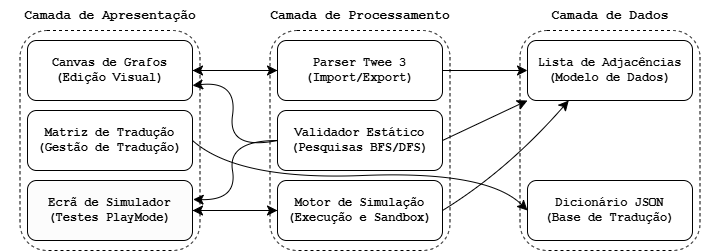
\includegraphics[width=0.9\linewidth]{Figures/arquitetura.png}
\caption{Diagrama de blocos detalhado da arquitetura conceptual e fluxo de dados.}
\label{fig:arquitetura-conceptual}
\end{figure}

\section{Requisitos do Sistema}
\label{sec:requisitos-sistema}

Com o intuito de delimitar o âmbito do projeto, o sistema foi estruturado para responder a necessidades fundamentais de modelação visual, internacionalização nativa, análise estática de integridade e inteligência artificial no cliente. Para a materialização prática do \gls{piap}, estas necessidades foram detalhadas sob a forma de requisitos técnicos, divididos entre funcionais (comportamento direto da aplicação) e não funcionais (restrições de qualidade, desempenho e usabilidade).

\subsection{Requisitos Funcionais}
\begin{description}
    \item[\textbf{RF01 - Criação e Edição de Nós Narrativos (Cenas):}] O utilizador deve poder instanciar, arrastar, atualizar (título e corpo de texto das cenas) e remover de forma atómica nós narrativos no canvas bidimensional.
    \item[\textbf{RF02 - Ligações Direcionadas entre Nós (Escolhas):}] O sistema deve inferir e instanciar arestas direcionadas automaticamente no grafo a partir da análise reativa de hiperligações double-bracket (\texttt{[[Texto|Destino]]}) inseridas pelo autor no texto das passagens.
    \item[\textbf{RF03 - Parser e Compatibilidade Twee 3:}] O sistema deve assegurar a interoperabilidade bidirecional síncrona com a especificação Twee 3, suportando a importação e exportação de ficheiros com extensão \texttt{.twee}, mantendo a sintaxe e efetuando o mapeamento geométrico das coordenadas espaciais dos nós.
    \item[\textbf{RF04 - Auditoria e Validação Estática de Fluxo:}] A plataforma deve executar análises estáticas e reativas sobre a topologia do grafo em plano secundário, sinalizando inconsistências estruturais como nós órfãos (inacessíveis), becos sem saída (hiperligações para identificadores inexistentes) ou caminhos inacessíveis devido a restrições lógicas.
    \item[\textbf{RF05 - Matriz de Localização Multi-idioma:}] O sistema deve disponibilizar uma matriz de tradução tabular centralizada que associe chaves dinâmicas das passagens a múltiplos dicionários de tradução, permitindo a exportação e importação síncrona de ficheiros em formato \gls{csv} em conformidade com a norma RFC 4180.
    \item[\textbf{RF06 - Simulador em Tempo Real (PlayMode):}] A aplicação deve integrar um simulador interativo em tempo real (\textit{PlayMode}) executado sob uma sandbox isolada do DOM, interpretando macros SugarCube, avaliando condições lógicas e executando scripts ou estilos customizados.
    \item[\textbf{RF07 - Zonas de Agrupamento Visual:}] O utilizador deve ser capaz de delimitar contêineres espaciais redimensionáveis (Zonas) para agrupamento lógico e organização de nós de cena, permitindo a sua translação conjunta no canvas.
    \item[\textbf{RF08 - Importação Inteligente via Conversor LLM:}] O sistema deve disponibilizar um assistente de inteligência artificial capaz de converter narrativas lineares em linguagem natural para o formato estruturado Twee 3, recorrendo à integração assíncrona com modelos de linguagem locais (Ollama) ou APIs externas.
\end{description}

\subsection{Requisitos Não Funcionais}
\begin{description}
    \item[\textbf{RNF01 - Portabilidade e Execução no Cliente (Browser):}] A plataforma deve ser executável inteiramente no lado do cliente através de um navegador de internet padrão, sem requerer servidores ou infraestruturas complexas.
    \item[\textbf{RNF02 - Usabilidade e Acessibilidade Visual:}] A interface de grafos deve utilizar a estética neo-brutalista e garantir que a visualização de fluxos (arestas de entrada e saída) seja distinguível sem dependência exclusiva de cor, apoiando utilizadores daltónicos.
    \item[\textbf{RNF03 - Desempenho e Fluidez:}] O canvas do React Flow e a conversão do parser síncrono devem suportar dezenas de nós em simultâneo com latência de interação e atualização abaixo de 100 milissegundos.
    \item[\textbf{RNF04 - Privacidade e Soberania de Dados:}] Todos os dados introduzidos, incluindo ficheiros importados, tabelas de tradução e dados submetidos para inteligência artificial no Ollama local, devem permanecer estritamente no armazenamento local do utilizador para garantir segurança absoluta.
\end{description}

\section{Métodos, Técnicas e Enquadramento Tecnológico}
\label{sec:metodos-tecnologia}

Para concretizar as especificações da arquitetura conceptual e responder aos requisitos definidos, o projeto apoia-se em metodologias ágeis de prototipagem rápida e numa seleção de tecnologias executadas do lado do cliente. As principais opções metodológicas e técnicas encontram-se estruturadas a seguir:

\begin{itemize}
    \item \textbf{Desenvolvimento da SPA (React 19) e Estilização (Tailwind CSS 3):}
    A aplicação foi inteiramente estruturada e programada pela equipa como uma \gls{spa} em \textbf{React 19} \citep{ReactReference}, tirando partido da nossa experiência prévia com esta tecnologia para gerir reativamente a árvore de componentes da interface. A identidade visual neo-brutalista (de alto contraste e bordas sólidas) foi desenhada e implementada por nós através da aplicação de classes utilitárias de \textbf{Tailwind CSS 3} \citep{TailwindCSSReference} nos componentes do editor.

    \item \textbf{Extensões ao Canvas de Grafos (ReactFlow 11):}
    Em vez de desenvolvermos um motor de desenho vetorial do zero, utilizámos a biblioteca \textbf{ReactFlow 11} \citep{ReactFlowReference} como base para gerir interações de zoom e arrasto. O nosso trabalho consistiu em estender esta infraestrutura básica através do desenvolvimento de nós totalmente customizados de cena (\texttt{StoryNode.jsx}) e de agrupamento (\texttt{ZoneNode.jsx}), além de arestas interativas personalizadas.

    \item \textbf{Algoritmia de Validação (Teoria de Grafos):}
    Concebemos e implementámos um modelo de dados baseado em listas de adjacências bidirecionais locais. Sobre esta estrutura, programámos algoritmos específicos para realizar análises topológicas em plano secundário (deteção de inconsistências via BFS) e a simulação de caminhos heurística do \textit{Smart Walker}.

    \item \textbf{Sistema de Internacionalização (i18next):}
    Integrámos a biblioteca \textbf{i18next} para gerir dicionários locais. Desenvolvemos o mapeamento que associa os dados tabulares da matriz de tradução do utilizador a ficheiros JSON de localização estáticos, carregados dinamicamente no navegador com o plugin de cliente \texttt{i18next-http-backend} sob o modelo \textit{backendless}.
\end{itemize}

\subsection{Justificação das Decisões de Design}
\label{subsec:justificacao-decisoes-design}
Com base na análise comparativa das ferramentas existentes (ver Secção~\ref{sec:analise-comparativa}), as escolhas de design e de tecnologia para o \gls{piap} foram fundamentadas nos seguintes pontos:
\begin{itemize}
    \item \textbf{Fusão de Paradigmas (Visual vs. Textual):} Enquanto o Twine se destaca pela interface puramente visual e o Ink pelo controlo fino de estados lógicos complexos, o \gls{piap} visa fundir ambas as forças, proporcionando um editor visual de grafos que não abdica da manipulação robusta de condicionais e variáveis (via macro-linguagem SugarCube).
    \item \textbf{Adoção do Formato Aberto Twee 3 e Limitação de Grafos:} A especificação aberta Twee 3 possui um mapeamento direto entre passagens e grafos, o que suporta a decisão de adotá-lo como base de persistência do \gls{piap}. Contudo, para permitir que o sistema leia as saídas e as renderize visualmente como arestas de forma fiável, o projeto introduz um compromisso de design (\textit{trade-off}) em relação ao Twine tradicional: não é suportada a utilização de variáveis como destinos dinâmicos de hiperligações (ex: \texttt{[[Ir para o local|\$local]]}), exigindo que todos os destinos do grafo sejam estáticos (conforme detalhado na Secção~\ref{subsec:destinos-dinamicos}).
    \item \textbf{Validação Automática e Segurança do Fluxo:} O ChoiceScript é valorizado pelas suas ferramentas robustas de teste automático (\texttt{randomtest}), uma lacuna crítica do Twine. O \gls{piap} incorpora de raiz este princípio ao disponibilizar o validador estático (\gls{bfs}) e o Smart Walker no simulador para preencher esta falta, garantindo a correção imediata do fluxo narrativo.
    \item \textbf{Autonomia e Licenciamento Livre:} A restrição de uso comercial imposta pelo ChoiceScript salienta a importância de desenvolver uma ferramenta que promova a autonomia dos autores, permitindo a exportação de projetos sob licenças livres e sem taxas adicionais.
\end{itemize}

\section{Modelação de Dados: Lista de Adjacência}
Para representar o fluxo da história no editor, o sistema utiliza uma \textbf{Lista de Adjacência Bidirecional}. Cada cena no modelo de dados armazena de forma independente dois conjuntos de caminhos:
\begin{itemize}
    \item \textbf{Saídas (Sucessores):} Um vetor que contém as escolhas explícitas disponíveis para o leitor, mapeando o texto da opção e o ID do nó de destino.
    \item \textbf{Entradas (Predecessores):} Um vetor que regista as referências de todos os outros nós que contêm escolhas a apontar para o nó atual.
\end{itemize}

Esta representação permite à aplicação realizar o mapeamento reverso instantâneo (\textit{backward mapping}), alimentando os painéis ``Vens de...'' e ``Vais para...'' na interface. A estrutura de dados \gls{json} representativa de um nó apresenta o seguinte formato simplificado:

\begin{code}
{
  "id": "cena_praca",
  "titulo": "A Praça Central",
  "conteudo": "O sol brilha no mercado central.",
  "saidas": [
    { "texto_escolha": "Entrar na taberna", "destino": "cena_taberna" }
  ],
  "entradas": ["cena_taberna"]
}
\end{code}

Note-se que este modelo foca-se exclusivamente na estrutura topológica do grafo. As variáveis globais e as condições lógicas SugarCube não são serializadas na lista de adjacências, sendo integradas diretamente no corpo de texto (\texttt{conteudo}) das passagens e interpretadas em tempo de execução pelo simulador.

\section{Parser Síncrono e Especificação Twee 3}
O ficheiro \texttt{tweeParser.js} (localizado em \texttt{/src/utils/tweeParser.js}) trata da sincronização bidirecional em tempo real entre o canvas do React Flow e o formato de texto Twee 3 \citep{Twee3Reference}.

Esta sincronização acontece de forma síncrona diretamente na memória do navegador. Isto significa que qualquer alteração de coordenadas, edição de texto ou criação de novas ligações no canvas é traduzida de imediato para a estrutura Twee 3 interna (e o oposto também se verifica), sem tempos de espera ou passos de compilação. Como a ferramenta funciona inteiramente no lado do cliente (\textit{client-side}), este mapeamento apenas mantém o estado da sessão atualizado; a persistência física dos dados no disco rígido requer sempre que o utilizador exporte o ficheiro de forma explícita.

\subsection{Importação e Conversão de Coordenadas de Zonas}
\label{subsec:conversao-coordenadas-zonas}
Durante a leitura e escrita de ficheiros, o parser converte as coordenadas de posição absolutas guardadas no formato Twee 3 (explicadas na Secção~\ref{subsec:metadados-tags-twee}) em coordenadas locais quando um nó é filho de uma Zona(explicado na Secção~\ref{subsec:zonas-agrupamento}). O React Flow exige que os nós filhos tenham posições relativas ao canto superior esquerdo da zona mãe, calculadas por:
\[
X_{\text{relativo}} = X_{\text{absoluto}} - X_{\text{zona}}
\]
\[
Y_{\text{relativo}} = Y_{\text{absoluto}} - Y_{\text{zona}}
\]
No processo inverso de exportação para ficheiro \texttt{.twee}, o parser executa a conversão inversa para manter a compatibilidade com outros compiladores de Twine:
\[
X_{\text{absoluto}} = X_{\text{zona}} + X_{\text{relativo}}
\]
\[
Y_{\text{absoluto}} = Y_{\text{zona}} + Y_{\text{relativo}}
\]

\subsection{Passagens Especiais}
O parser reconhece passagens reservadas de metadados da especificação Twee 3:
\begin{itemize}
    \item \texttt{:: StoryTitle}: Define o título do projeto.
    \item \texttt{:: StoryData}: Contém as configurações globais em formato \gls{json}, incluindo o identificador único da história (\texttt{ifid}), o formato de compilação (\texttt{SugarCube}), o nó de arranque (\texttt{start}) e o nível de zoom.
    \item \texttt{:: StoryInit}: Nó especial não-narrativo onde são declaradas e inicializadas as variáveis lógicas de controlo do estado da simulação (as quais servem de memória do jogo, conforme introduzido na Secção~\ref{sec:arquitetura-geral}).
\end{itemize}

\subsection{Modelo SugarCube (Ligações e Macros)}
As arestas são extraídas do texto narrativo de cada nó através de expressões regulares que identificam ligações no formato clássico Twee:
\begin{itemize}
    \item \textbf{Arestas Simples:} \texttt{[[Cena2]]}
    \item \textbf{Arestas com Alias ou Direcionamento:} \texttt{[[Ir para a Taverna|cena\_taberna]]} ou \texttt{[[Abrir porta->cena\_interior]]}
\end{itemize}

No caso das macros de alteração de estado (ex: \texttt{<<set \$moedas += 10>>}) e condicionais lógicas (ex: \texttt{<<if \$tem\_chave>> ... <</if>>}), o parser de importação não as compila nem as remove do texto. O parser executa duas operações:
\begin{enumerate}
    \item \textbf{Preservação de Código:} Mantém as macros intactas no corpo textual da passagem, permitindo que sejam interpretadas e executadas reativamente pelo simulador (\textit{PlayMode}) durante a execução do jogo (ver Secção~\ref{subsec:compilador-jit-macros}).
    \item \textbf{Extração de Variáveis para Indexação:} Identifica os nomes das variáveis (iniciadas por \texttt{\$}) e regista-as no painel de gestão de variáveis, permitindo que o autor as rastreie ou renomeie de forma atómica em todo o projeto.
\end{enumerate}

\section{Interação Visual, Edição e Acessibilidade}

\subsection{Zonas de Agrupamento Visual}
\label{subsec:zonas-agrupamento}
As \textbf{Zonas de Agrupamento Visual} (\texttt{ZoneNode}) consistem em contentores espaciais retangulares que agrupam logicamente nós de cena relacionados (como capítulos ou localizações), conforme ilustrado na Figura~\ref{fig:exemplo-zona}.

\begin{figure}[H]
    \centering
    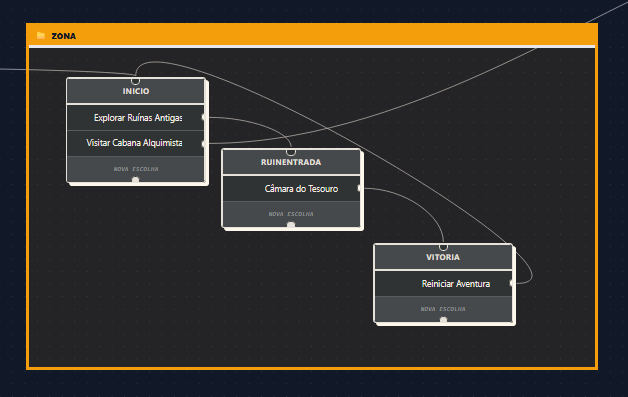
\includegraphics[width=0.65\textwidth]{Figures/zone.png}
    \caption{Exemplo de uma Zona de Agrupamento Visual com nós de cena filhos no canvas.}
    \label{fig:exemplo-zona}
\end{figure}

A sua implementação como nós de grupo personalizados exigiu contornar um problema de colisão de cliques no React Flow. Como o contentor cobre uma área retangular considerável sobreposta aos nós de cena interiores, os \textit{pointer events} capturavam os cliques no ecrã, impedindo a seleção ou arrasto dos filhos. Para resolver isto, definiu-se a propriedade CSS \texttt{pointer-events: none} dinamicamente na configuração global do React Flow para o contentor da Zona em \texttt{App.jsx}. Em paralelo, no componente \texttt{ZoneNode.jsx}, forçou-se \texttt{pointer-events: auto} exclusivamente nas pegas de redimensionamento (\textit{NodeResizer}) e na barra de cabeçalho (utilizada para arrastar a zona em bloco com todos os seus filhos).

As Zonas suportam ainda imagens de fundo personalizadas (\textit{backgrounds}) geridas através da propriedade reativa \texttt{bgImage} nos metadados do nó, a qual é descodificada em tempo de execução e aplicada via CSS.

\subsection{Arestas Curvadas com Waypoints}
\label{subsec:arestas-curvadas-waypoints}

Para evitar a sobreposição visual das ligações e o cruzamento cego sobre os nós de cena, a plataforma implementa arestas personalizadas que utilizam a interpolação por \textit{Splines} Cúbicas de Catmull-Rom \citep{CatmullRom1974}. Esta lógica encontra-se implementada no componente \texttt{EditableEdge.jsx} (\texttt{/src/components/EditableEdge.jsx}), com o resultado visual exemplificado na Figura~\ref{fig:curved-edge}.

\begin{figure}[H]
    \centering
    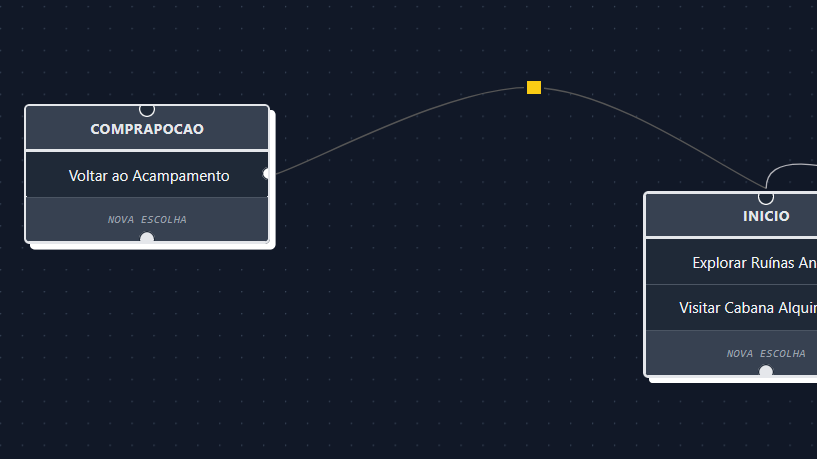
\includegraphics[width=0.65\textwidth]{Figures/curved_edge.png}
    \caption{Exemplo de aresta suavizada com caminho curvado personalizável no canvas.}
    \label{fig:curved-edge}
\end{figure}

O autor pode criar novos marcadores (\textit{waypoints}) com um duplo clique e arrastá-los livremente pelo ecrã. A curva é recalculada em tempo de execução à medida que os marcadores são movidos, interpolando a sua posição de forma contínua para manter a linha fluida e desimpedida de outros elementos do grafo.

\subsection{Acessibilidade e Identidade Visual Customizada}
\label{subsec:acessibilidade-identidade-visual}
Tendo em conta que o desenvolvimento do projeto beneficiou de validações diretas com utilizadores daltónicos, projetou-se uma estratégia de acessibilidade redundante baseada numa identidade visual neo-brutalista. A adoção desta estética neo-brutalista fundamentou-se em estudos que demonstram que contornos espessos, pesos tipográficos elevados e contrastes marcados beneficiam utilizadores com baixa acuidade visual ou daltonismo \citep{Babich2023, Loranger2022}. O aspeto geral desta interface e os seus elementos gráficos encontram-se representados na Figura~\ref{fig:editor-canvas-acessibilidade}.

\begin{figure}[H]
    \centering
    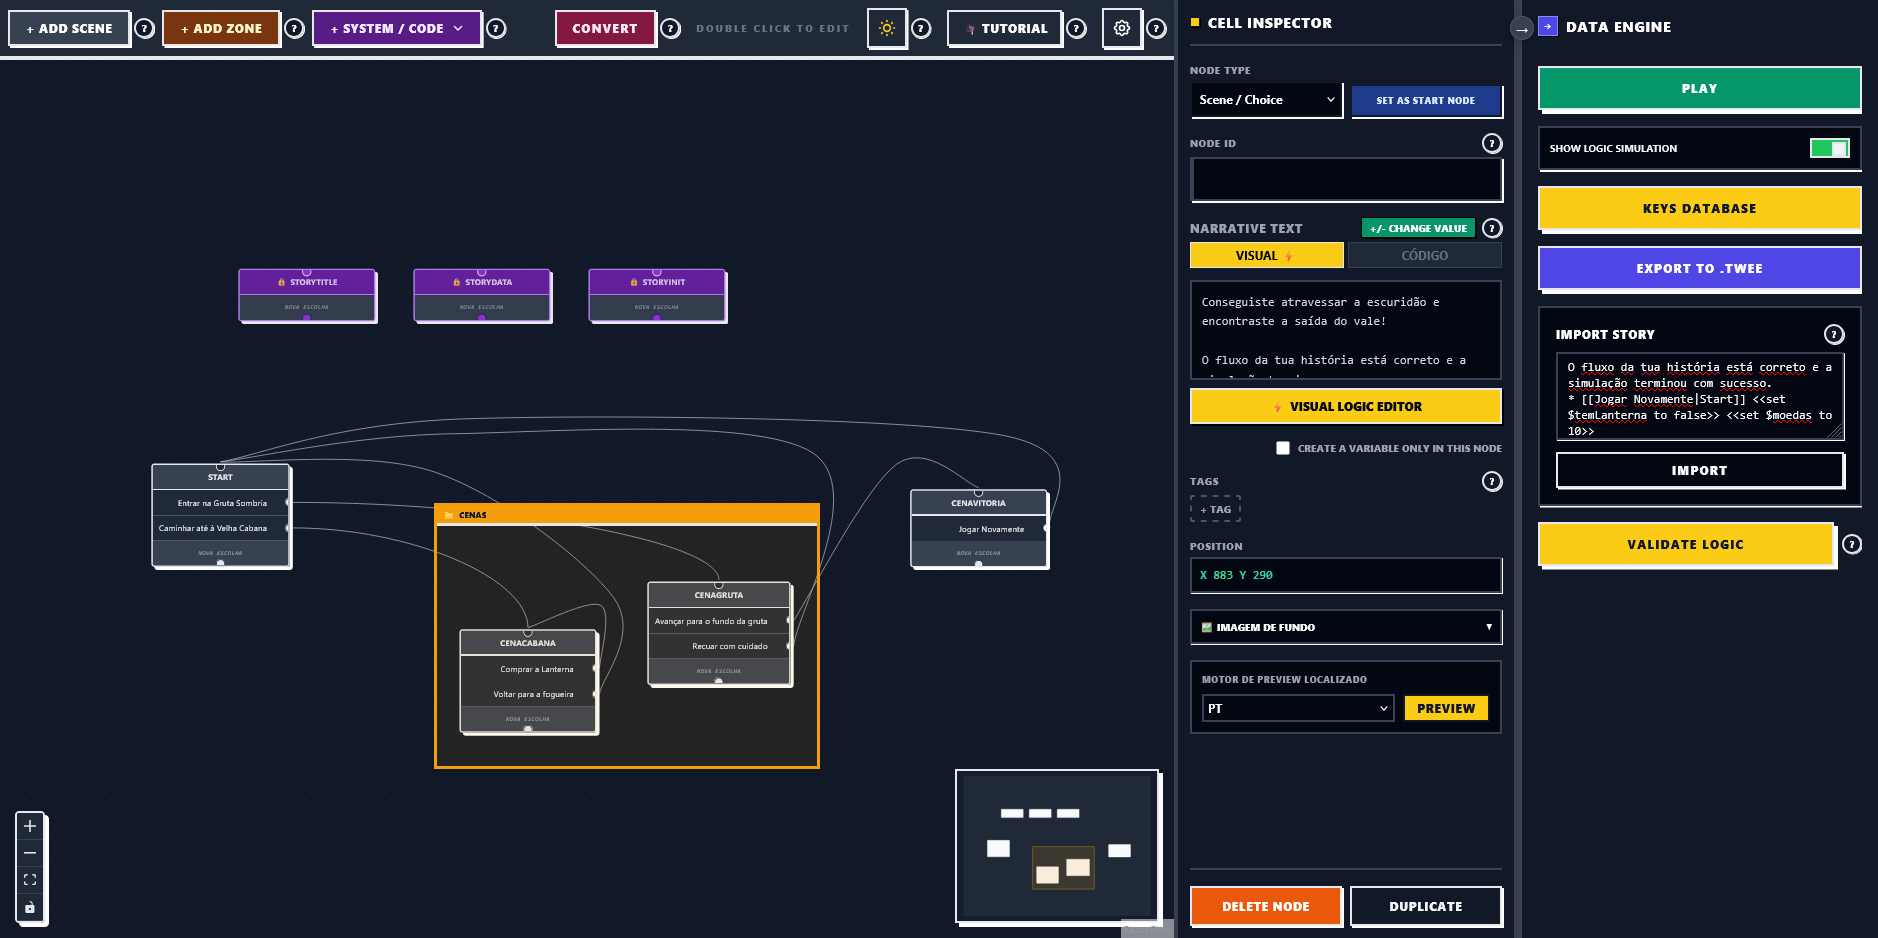
\includegraphics[width=0.85\textwidth]{Figures/editor_canvas.png}
    \caption{Interface gráfica global do editor (\textit{Plot in a Pot}), ilustrando a identidade visual neo-brutalista de alto contraste com contornos espessos e sinalização redundante para acessibilidade.}
    \label{fig:editor-canvas-acessibilidade}
\end{figure}

O nosso trabalho de design e programação focou-se nos seguintes pilares:
\begin{itemize}
    \item \textbf{Delimitação por Contornos Sólidos:} Implementação de contornos pretos de 2px (\texttt{border-2}) e sombras projetadas rígidas sem difusão (\texttt{shadow-[4px\_4px\_0px\_\#000]}) em todos os componentes visuais (\textit{StoryNode}, \textit{ZoneNode} e painéis), eliminando a dependência de cores ou gradientes suaves para distinguir elementos.
    \item \textbf{Diferenciação Estrutural de Arestas:} As transições normais no grafo são desenhadas com traçados contínuos, enquanto as ligações inacessíveis ou com erros lógicos são renderizadas com traçados tracejados (\texttt{strokeDasharray="5,5"}). Esta distinção de padrão garante que o utilizador consiga identificar caminhos quebrados sem depender exclusivamente da cor.
    \item \textbf{Sinalização Semântica Dupla de Alertas:} Configuração de etiquetas textuais explícitas (como o selo ``Aviso'' em fundo laranja nos nós com erros estruturais) em conjunto com listagens descritivas nos painéis, evitando a sinalização baseada apenas no par de cores verde/vermelho.
\end{itemize}

\subsection{Modelação de Dados e Sincronização com o React Flow}
\label{subsec:modelacao-dados-reactflow}
Para além da representação abstrata da arquitetura, a implementação prática exige uma sincronização bidirecional em tempo real entre a interface gráfica gerida pela biblioteca \textit{React Flow} e a estrutura de dados semântica interna da história.

No \gls{piap}, o estado centralizado da narrativa é mantido na raiz da aplicação (\texttt{App.jsx}) e de forma modular através de ganchos personalizados (\textit{custom hooks}), recorrendo a três vetores de dados estruturados em memória local:
\begin{enumerate}
    \item \textbf{Vetor de Nós do React Flow (\texttt{nodes}):} Contém a representação posicional e de renderização de cada elemento no canvas. Cada objeto de nó segue a especificação rígida da biblioteca:
\begin{verbatim}
{
  id: "cena_taberna",
  type: "storyNode",
  position: { x: 250, y: 180 },
  data: {
    title: "Interior da Taberna",
    content: "O cheiro a hidromel preenche a sala...",
    tags: ["secreto"],
    bgImage: ""
  },
  width: 280,
  height: 150
}
\end{verbatim}
    Se o nó representar uma Zona de Agrupamento (\texttt{ZoneNode}), o tipo é alterado para \texttt{"zoneNode"} e o objeto passa a incluir propriedades de agrupamento como \texttt{parentId} nos nós filhos e dimensões explícitas de largura e altura controladas pelo utilizador.
    
    \item \textbf{Vetor de Arestas do React Flow (\texttt{edges}):} Modela a conectividade geométrica das escolhas narrativas. Cada aresta é configurada como um componente personalizado (\texttt{EditableEdge}) e armazena os pontos geométricos intermédios (\textit{waypoints}) inseridos pelo autor para suavizar as curvas:
\begin{verbatim}
{
  id: "edge-cena_praca-cena_taberna",
  source: "cena_praca",
  target: "cena_taberna",
  type: "editableEdge",
  data: {
    choiceText: "Entrar na taberna",
    waypoints: [{ x: 120, y: 150 }, { x: 180, y: 160 }]
  }
}
\end{verbatim}
    
    \item \textbf{Lista de Adjacência Bidirecional (\texttt{adjacencyList}):} Representa o grafo direcionado de estados do ponto de vista do motor lógico. É recalculada de forma síncrona a cada modificação nos vetores de nós ou arestas. Esta lista mapeia cada identificador de cena ao seu conjunto de sucessores (saídas) e predecessores (entradas), permitindo ao validador e ao motor de simulação executar travessias e pesquisas rápidas.
\end{enumerate}

Esta tripla modelação é sincronizada de forma atómica. Quando o autor arrasta um nó ou altera o texto de uma escolha no painel de detalhes, os manipuladores de eventos reativos do React Flow (como \texttt{onNodesChange} ou \texttt{onEdgesChange}) capturam a alteração física. Esta alteração é processada e encaminhada pelos ganchos personalizados em \texttt{App.jsx}, gerando novos vetores imutáveis de estado que forçam a atualização dos componentes visuais e o recálculo imediato da lista de adjacências e do mapa de erros lógicos.

\section{Validação Estática e Simulação}
\label{sec:validacao-estatica-simulacao}

O motor de autoria do \textit{Plot in a Pot} integra ferramentas robustas de validação e execução reativa. Para além de permitir a escrita de histórias, a plataforma disponibiliza um sistema de verificação lógica que audita a estrutura narrativa de forma estática e uma sandbox de simulação dinâmica dotada de agentes de navegação autónoma.

\subsection{Algoritmo de Validação Estática e Exploração do Espaço de Estados (\gls{bfs})}
\label{subsec:algoritmo-bfs-validacao}

O validador estático, implementado em \texttt{storyValidator.js} e \texttt{storyTraversal.js}, resolve o problema de acessibilidade e integridade da narrativa. Em grafos estáticos simples, uma travessia clássica de Pesquisa em Largura (\gls{bfs}) seria suficiente para auditar o grafo. Contudo, em \gls{ni}, as arestas (hiperligações) dependem frequentemente de expressões lógicas e variáveis de estado (macros \texttt{<<if>>} e \texttt{<<set>>} do SugarCube). A acessibilidade de um nó $v$ não depende apenas do caminho geométrico, mas também da valoração atual das variáveis de estado (memória).

Assim, a validação lógica é modelada como um problema de \textit{Exploração do Espaço de Estados} (\textit{State Space Exploration}), onde o grafo de transições real é constituído por pares $\langle v, \sigma \rangle$, nos quais $v \in \mathcal{N}$ representa o nó do editor e $\sigma: \mathcal{V} \rightarrow \mathcal{D}$ representa um mapeamento de variáveis lógicas globais para os seus respetivos domínios de valores.

O algoritmo executa a travessia de acordo com os seguintes passos estruturados:

\begin{enumerate}
    \item \textbf{Inicialização e Pré-computação:}
    Para garantir a eficiência temporal ($\mathcal{O}(1)$ em lookups), o algoritmo pré-computa em memória:
    \begin{itemize}
        \item Um mapa de nós $NodeMap: \text{ID} \rightarrow Node$, indexando todos os vértices da narrativa.
        \item Um mapa de adjacências de arestas $EdgesBySource: \text{ID} \rightarrow List\langle Edge \rangle$.
    \end{itemize}
    O ponto de entrada $v_0$ é resolvido por $findStartNode(NodeMap)$, e o estado inicial $\sigma_0$ é lido a partir das declarações de variáveis do nó de sistema $StoryInit$.
    
    \item \textbf{Estrutura de Dados e Fila:}
    Uma fila síncrona $\mathcal{Q}$ é instanciada e inicializada com o tuplo de arranque:
    \[
    \mathcal{Q} \leftarrow \text{enqueue}\left(\mathcal{Q}, \langle v_0, \sigma_0, \text{path} = [v_0.\text{label}] \rangle\right)
    \]
    São criados conjuntos vazios para registar nós alcançáveis ($\mathcal{N}_{reach}$), arestas alcançáveis ($\mathcal{E}_{reach}$), e tabelas hash de estados visitados por nó ($VisitedStates: \text{ID} \rightarrow Set\langle String \rangle$) para evitar caminhos redundantes e ciclos infinitos.
    
    \item \textbf{Ciclo de Processamento Principal:}
    Enquanto $\mathcal{Q}$ não estiver vazia, remove-se o primeiro elemento:
    \[
    \langle u, \sigma, \text{path} \rangle \leftarrow \text{dequeue}(\mathcal{Q})
    \]
    Para o nó corrente $u$, efetua-se o seguinte processamento:
    \begin{enumerate}
        \item Adiciona-se o identificador de $u$ a $\mathcal{N}_{reach}$.
        \item Executam-se as instruções de modificação de estado contidas no texto do nó (por exemplo, macros de atribuição \texttt{<<set>>}), produzindo um novo estado de memória $\sigma' \leftarrow applyModifiers(u.\text{content}, \sigma)$.
        \item Verifica-se se o estado $\sigma'$ já foi visitado no nó $u$. Para tal, converte-se $\sigma'$ numa representação string serializada $S_{\sigma'}$ e verifica-se se $S_{\sigma'} \in VisitedStates[u]$. Em caso afirmativo, o ramo é podado (\textit{pruning}) para evitar ciclos redundantes no grafo.
        \item Para evitar a explosão do espaço de estados em loops que incrementam variáveis infinitamente, impõe-se um limite de segurança de $K = 10$ estados únicos por nó. Se $|VisitedStates[u]| \ge K$, o algoritmo emite um aviso de ciclo infinito no terminal e poda o caminho.
        \item Caso contrário, insere-se $S_{\sigma'}$ em $VisitedStates[u]$ e regista-se a rota percorrida e o estado final na tabela de histórico de chegada $ArrivalHistory[u]$.
    \end{enumerate}
    
    \item \textbf{Avaliação de Transições e Condicionais:}
    Para cada aresta de saída $e \in EdgesBySource[u]$ que conecta o nó $u$ ao nó de destino $w$:
    \begin{enumerate}
        \item O validador extrai a hiperligação textual associada à aresta $e$ do conteúdo de $u$.
        \item Avalia-se a condição de acessibilidade associada a essa escolha através da função $canAccessChoice(u.\text{content}, \text{link}, \sigma')$. Esta função analisa se o link está envolto por alguma macro condicional \texttt{<<if>>} e avalia a sua expressão lógica contra a memória $\sigma'$.
        \item Se a condição for satisfeita ($true$), adiciona-se o ID da aresta $e$ a $\mathcal{E}_{reach}$ e enfileira-se o próximo estado:
        \[
        \mathcal{Q} \leftarrow \text{enqueue}\left(\mathcal{Q}, \langle w, \sigma', \text{path} \cup [w.\text{label}] \rangle\right)
        \]
    \end{enumerate}
\end{enumerate}

Após o término da travessia (quando a fila $\mathcal{Q}$ fica vazia), o módulo de auditoria em \texttt{storyValidator.js} pós-processa os resultados recolhidos para isolar as falhas estruturais, categorizando-as em:
\begin{itemize}
    \item \textbf{Nós Órfãos ($V_{orphan}$):} Nós $v \in \mathcal{N}$ que não pertencem a $\mathcal{N}_{reach}$ e cujas etiquetas não incluem a tag \texttt{''secreto''}.
    \item \textbf{Becos sem Saída ($V_{dead\_end}$):} Nós $v \in \mathcal{N}_{reach}$ que contêm hiperligações cujo destino aponta para um ID de nó inexistente no grafo ($w \notin \mathcal{N}$).
    \item \textbf{Arestas Inacessíveis ($E_{unreachable}$):} Arestas $e \in \mathcal{E}$ que não pertencem a $\mathcal{E}_{reach}$. Estas representam caminhos cujas condicionais lógicas nunca são satisfeitas sob nenhuma das valorações de variáveis exploradas.
\end{itemize}

\subsection{Simulador em Tempo Real (PlayMode) e Smart Walker}
\label{subsec:simulador-playmode-walker}

O simulador de jogo (\texttt{PlayMode.jsx}) mimetiza o comportamento do interpretador SugarCube num ambiente controlado pelo navegador do autor. Para permitir a depuração em tempo real sem afetar os dados de edição, o motor executa sob um isolamento de contextos:
\begin{itemize}
    \item \textbf{Separação de Estilos:} Os nós categorizados com a tag \texttt{css} têm o seu conteúdo concatenado em tempo de execução e injetado sob a forma de uma tag \texttt{<style id=''playmode-styles''>} na raiz do cabeçalho da página, sendo totalmente limpos ao sair da simulação.
    \item \textbf{Isolamento de Scripts:} Os nós lógicos contendo JavaScript são processados como funções anónimas com escopo isolado através do construtor \texttt{new Function('state', 'State', 'setup', script\_content)}, impedindo que variáveis globais escritas pelo utilizador interfiram com os estados internos do React ou do canvas do React Flow.
\end{itemize}

Para testes automáticos de caminhos narrativos, a plataforma disponibiliza o agente autónomo \textbf{Smart Walker} (implementado em \texttt{storyTraversal.js}). Em vez de selecionar opções de forma puramente pseudo-aleatória (o que levaria a uma baixa cobertura de caminhos e retenção em ciclos curtos), o agente utiliza uma heurística baseada em \textit{Procura por Novidade} (\textit{Novelty Search}).

Dada a vizinhança do nó atual $v$, correspondente ao conjunto de nós adjacentes alcançáveis $N(v)$, o agente consulta o histórico de visitas acumuladas do simulador. Para cada opção de transição que leva ao nó vizinho $w \in N(v)$, o Smart Walker obtém o número acumulado de visitas históricas $H(w)$ registado na memória global do simulador. O Walker seleciona a transição para o nó vizinho $w_{next}$ que minimiza a frequência de visitas:
\[
w_{next} = \arg\min_{w \in N(v)} H(w)
\]
Este comportamento força o simulador a procurar caminhos narrativos raros e ramos profundos da história de forma automatizada, conseguindo mapear e encontrar becos sem saída ou ciclos lógicos fechados numa fração de segundo sem intervenção manual do autor.

\subsection{Motor de Compilação JIT de Macros SugarCube}
\label{subsec:compilador-jit-macros}

Para suportar as avaliações e atribuições de variáveis de estado descritas, a aplicação possui um compilador \textit{Just-In-Time} (JIT) simplificado estruturado em \texttt{logicParser.js} e \texttt{sugarcubeLogic.js}:
\begin{itemize}
    \item \textbf{Análise Léxica e Mapeamento:} O interpretador analisa o conteúdo textual dos nós através de varrimentos que procuram padrões de macros \texttt{<<set>>} e \texttt{<<if>>}. Traduz os operadores clássicos da linguagem SugarCube para os operadores lógicos válidos de JavaScript, conforme resumido na Tabela~\ref{tab:operadores-sugarcube}.
    \item \textbf{Árvore de Sintaxe Abstrata (\gls{ast}):} O interpretador de condicionais analisa blocos lógicos aninhados construindo uma \gls{ast} simples que reflete a precedência de cláusulas. Esta estrutura é então avaliada em tempo de execução para calcular o valor de verdade das expressões.
\end{itemize}

\begin{table}[htbp]
    \centering
    \caption{Mapeamento de operadores lógicos SugarCube para JavaScript.}
    \label{tab:operadores-sugarcube}
    \begin{tabular}{lll}
        \toprule
        \textbf{Operador SugarCube} & \textbf{Operador JavaScript} & \textbf{Significado} \\
        \midrule
        \texttt{is} / \texttt{eq} & \texttt{===} & Igualdade estrita \\
        \texttt{neq} & \texttt{!==} & Diferença estrita \\
        \texttt{and} & \texttt{\&\&} & E lógico \\
        \texttt{or} & \texttt{||} & OU lógico \\
        \texttt{to} & \texttt{=} & Atribuição de valor \\
        \texttt{\$variavel} & \texttt{state.variavel} & Acesso ao estado reativo \\
        \bottomrule
    \end{tabular}
\end{table}

\section{Integração de Modelos de Linguagem (LLMs)}
\label{sec:integracao-llms-implementacao}
Para além do núcleo lógico de grafos e da simulação estática, a plataforma disponibiliza um assistente baseado em Modelos de Linguagem de Grande Escala (LLMs) para facilitar a importação e co-criação de histórias. A conceção e implementação desta funcionalidade assenta nos seguintes aspetos:

\subsection{Arquitetura de Integração Local}
A integração com inteligência artificial foca-se em fornecer uma interface de comunicação local e assíncrona entre o editor gráfico e o servidor de inferência do utilizador. O trabalho de desenvolvimento realizado pela equipa consistiu em:
\begin{itemize}
    \item \textbf{Módulo de Comunicação REST (\texttt{aiGenerator.js}):} Programámos o cliente HTTP em Javascript para estabelecer a ligação assíncrona com o endpoint local do Ollama (\texttt{http://localhost:11434}), enviando os cabeçalhos e o corpo JSON com os parâmetros de temperatura e tokens.
    \item \textbf{Engenharia de Prompt de Conversão:} Desenvolvemos e validámos um prompt de sistema especializado, com regras sintáticas rígidas, concebido para forçar o modelo de linguagem a gerar respostas estritamente em conformidade com a especificação Twee 3 (cabeçalhos, metadados e arestas literais), mitigando alucinações.
    \item \textbf{Importação Automatizada Pós-Resposta:} Desenvolvemos o fluxo de importação que recebe o texto estruturado retornado pela API local, encaminha-o para o nosso parser e gera automaticamente os nós e arestas correspondentes no canvas.
\end{itemize}

A decisão de basear este assistente em inferência local (via Ollama) assenta nos seguintes compromissos:
\begin{itemize}
    \item \textbf{Privacidade e Soberania dos Dados:} Ao executar o modelo localmente no computador do autor, garante-se que toda a propriedade intelectual da história e os textos criados permanecem estritamente confidenciais. Não há partilha de dados com servidores externos de terceiros nem risco de os textos literários serem recolhidos para treino de modelos comerciais.
    \item \textbf{Custo Financeiro Zero:} APIs na nuvem implicam faturação contínua baseada em consumo de tokens, o que criaria barreiras ao uso regular. A inferência local permite a utilização gratuita e ilimitada da funcionalidade de conversão inteligente.
\end{itemize}

\subsection{Papel do LLM: Conversão e Importação Automática de Histórias}
A nossa abordagem de design delimitou de forma clara o papel do modelo de linguagem no ciclo de vida da narrativa. Visto que os LLMs tendem a alucinar, criar caminhos impossíveis e ignorar restrições de ciclos, o modelo não é integrado dinamicamente na simulação direta do jogo.

O papel do LLM foi desenhado por nós para atuar estritamente como uma ferramenta de conversão sintática em fase de pré-processamento. O modelo lê a história linear fornecida pelo autor e converte-a para a norma Twee 3. A partir desse ponto, o nosso motor lógico e o validador BFS assumem a responsabilidade exclusiva de renderizar o canvas visual e garantir a integridade dos caminhos e das variáveis de estado no editor.



\chapter{Implementação e Avaliação}
\label{cp:desenvolvimento}

Este capítulo detalha o processo de implementação prática do \textit{Plot in a Pot}, descrevendo a estrutura física do código, detalhes de componentes e utilitários, testes lógicos de inteligência artificial, benchmarks de desempenho e a metodologia e resultados dos testes de utilizador realizados para validar o sistema.

\section{Estrutura do Código e Detalhes de Implementação}
\label{sec:estrutura-codigo-implementacao}

Para além da fundamentação teórica, o processo de desenvolvimento envolveu a estruturação de uma base de código robusta, modular e altamente reativa. O software está organizado de forma a garantir a separação de conceitos (\textit{Separation of Concerns}), dividindo-se entre componentes de interface visuais, ganchos customizados (\textit{custom hooks}) e utilitários de processamento lógico puro.

\subsection{Gestão de Estado Global, Reatividade e Histórico}
O componente principal \texttt{App.jsx} atua como o orquestrador reativo central do sistema. Para evitar a criação de um ficheiro monolítico, a equipa encapsulou a lógica de negócio em ganchos customizados (\textit{custom hooks}) específicos:
\begin{itemize}
    \item \textbf{\texttt{useSettings}:} Centraliza o estado e a persistência em \textit{LocalStorage} das opções de visualização (ex: exibição de erros, nós secretos, e grau de desfocagem da imagem de fundo).
    \item \textbf{\texttt{useUndoRedo}:} Controla as pilhas de estados anteriores (\texttt{past}) e futuros (\texttt{future}) para as operações atómicas de desfazer e refazer no canvas.
    \item \textbf{\texttt{useChoiceSync}:} Implementa a análise sintática em tempo real para sincronizar as ligações textuais com as arestas correspondentes a escolhas.
    \item \textbf{\texttt{useNodeOperations}:} Encapsula a criação, remoção, duplicação e atualização de propriedades semânticas e posicionais de nós e zonas no editor.
    \item \textbf{\texttt{useGraphHandlers}:} Gere as interações gráficas ligadas ao canvas (ligar nós, atualizar arestas, gerir arrasto e inserção em zonas de agrupamento).
    \item \textbf{\texttt{useKeyboardShortcuts}:} Escuta eventos do teclado para acionar atalhos de produtividade global.
    \item \textbf{\texttt{useProjectPersistence}:} Controla a gravação automática periódica, tradução em tempo real, importação bidirecional de ficheiros Twee 3 e carregamento de modelos base.
\end{itemize}

A implementação do histórico colocou um desafio relevante no contexto de reatividade do React. Como o React Flow atualiza objetos de nós e arestas por referência, a simples inserção de estados na pilha de histórico resultaria na mutação dos estados passados sempre que o utilizador arrastasse um nó. Para resolver esta limitação, implementou-se uma estratégia de clonagem profunda (\textit{deep clone}) em cada instantâneo, conforme demonstrado na Listagem~\ref{lst:app-undo-redo}.

\begin{listing}[H]
\begin{lstlisting}
// Registo de snapshots e funcoes de controlo em useUndoRedo.js
const takeSnapshot = useCallback(() => {
  setPast(prev => [
    ...prev.slice(-50),
    {
      nodes: JSON.parse(JSON.stringify(nodesRef.current)),
      edges: JSON.parse(JSON.stringify(edgesRef.current))
    }
  ]);
  setFuture([]);
}, []);

const undo = useCallback(() => {
  if (past.length === 0) return;
  const previous = past[past.length - 1];
  setFuture(prev => [
    {
      nodes: JSON.parse(JSON.stringify(nodesRef.current)),
      edges: JSON.parse(JSON.stringify(edgesRef.current))
    },
    ...prev
  ]);
  setPast(prev => prev.slice(0, -1));
  setNodes(previous.nodes);
  setEdges(previous.edges);
}, [past]);
\end{lstlisting}
\caption{Mecanismo de clonagem profunda e gestão da pilha de histórico encapsulado em useUndoRedo.js.}
\label{lst:app-undo-redo}
\end{listing}

Esta estrutura suporta o fluxo reativo unidirecional da aplicação. Quando o autor edita o texto de uma passagem no painel de propriedades, um evento de alteração é propagado para o estado central em \texttt{App.jsx}, que força a reavaliação síncrona e em segundo plano de dois subsistemas independentes: o parser de texto (que extrai as novas arestas baseadas em ligações double-bracket e reconstrói a Lista de Adjacência em memória) e o validador estático (que executa a travessia BFS sobre a nova lista de adjacência para detetar inconsistências e desenhar alertas visuais de aviso diretamente no canvas).

\subsection{Componentes Gráficos e Desafios de Interação (Canvas, Nós e Arestas)}
Os nós gráficos que habitam o canvas estendem os componentes base da biblioteca React Flow (conforme ilustrado na Figura~\ref{fig:editor-canvas}):
\begin{itemize}
    \item \textbf{StoryNode.jsx:} Renderiza o título da passagem, o extrato de texto da história e as portas de ligação (\textit{handles}) de entrada e saída.
    \item \textbf{ZoneNode.jsx (Agrupamento Visual):} Implementa o agrupamento de capítulos. Para resolver o conflito de eventos de rato (onde a Zona sobreposta impedia cliques no canvas de fundo ou nos nós filhos), aplicou-se a propriedade CSS \texttt{pointer-events: none} ao contêiner geral da Zona, e ativou-se \texttt{pointer-events: all} exclusivamente para as bordas de redimensionamento e barra de cabeçalho, como demonstrado na Listagem~\ref{lst:zone-pointer-events}.
    \item \textbf{EditableEdge.jsx (Arestas Curvas):} Implementa o traçado curvo interativo. O utilizador pode efetuar um duplo clique sobre a linha para introduzir um ponto de controlo (\textit{waypoint}) geométrico. O algoritmo (Listagem~\ref{lst:edge-path-svg}) interpola os pontos e converte a spline Catmull-Rom em comandos de curva Bézier cúbica SVG (\texttt{C}) compatíveis com o navegador.
\end{itemize}

\begin{figure}[H]
    \centering
    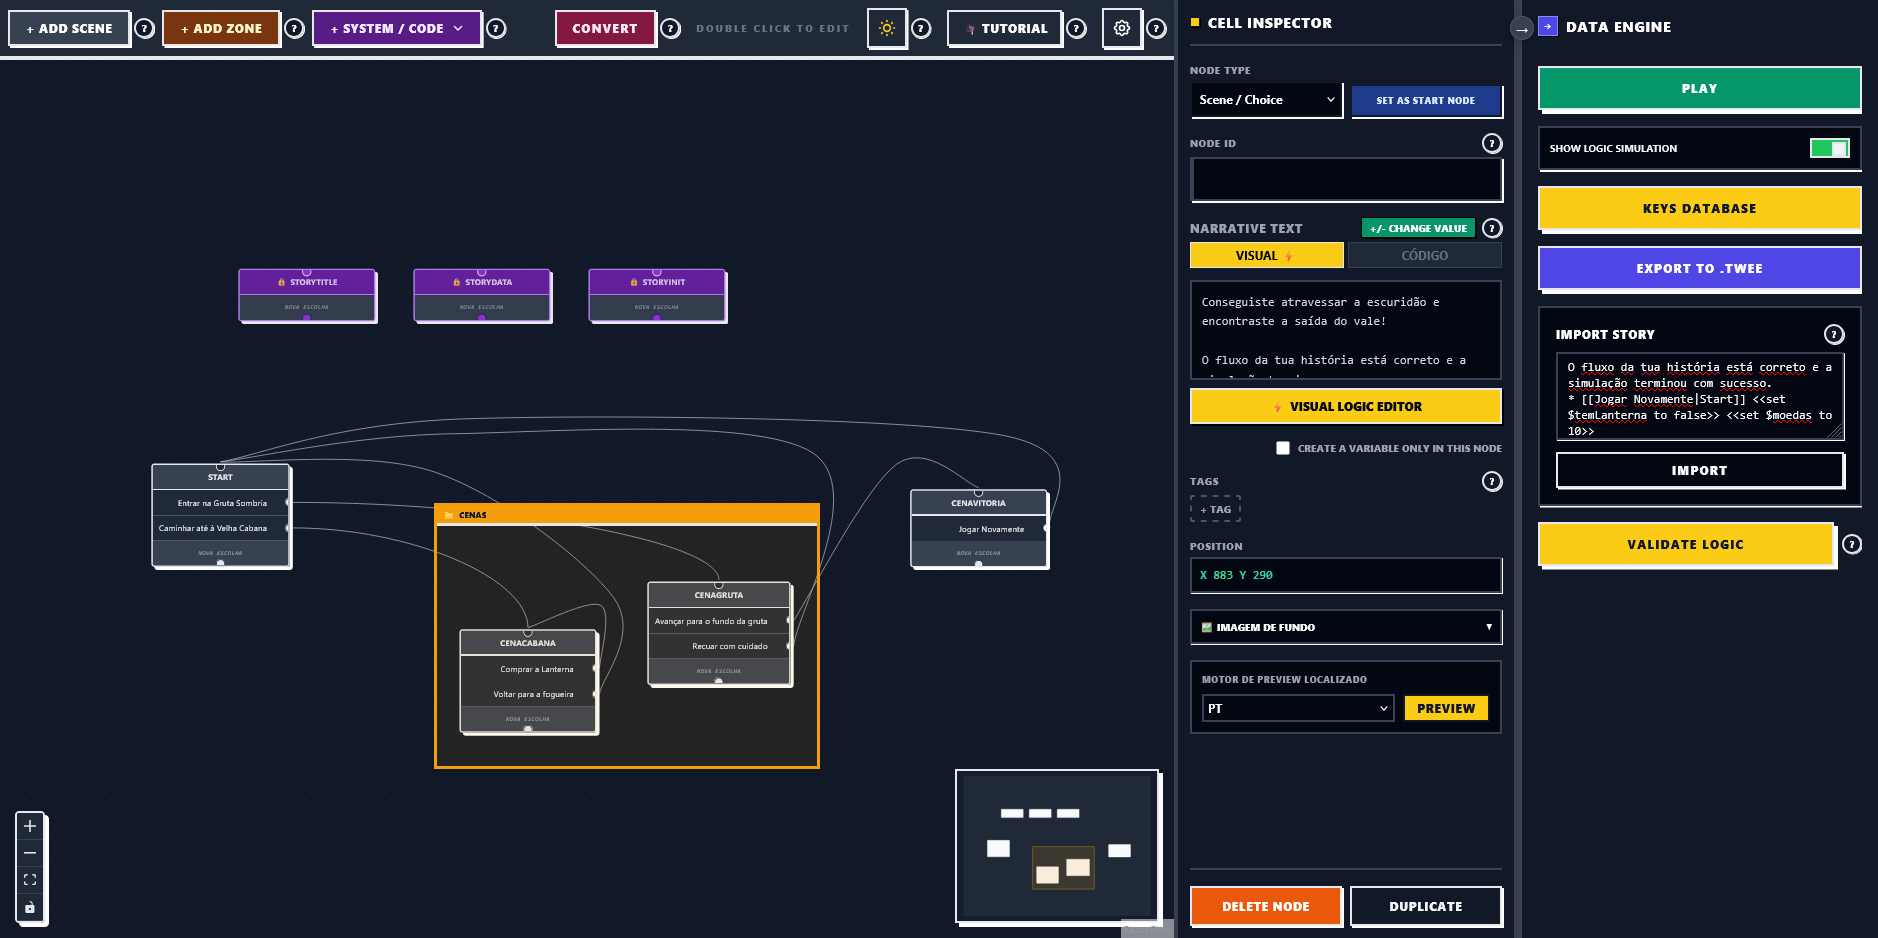
\includegraphics[width=0.85\linewidth]{Figures/editor_canvas.png}
    \caption{Interface gráfica do canvas de grafos do Plot in a Pot, demonstrando a estética neo-brutalista de alto contraste com nós de cena e agrupamentos visuais (Zonas).}
    \label{fig:editor-canvas}
\end{figure}

\begin{listing}[H]
\begin{lstlisting}
<!-- Estrutura simplificada do componente ZoneNode -->
<div 
  className="zone-node-container" 
  style={{ pointerEvents: 'none' }}
>
  <div 
    className="zone-node-header" 
    style={{ pointerEvents: 'all' }}
  >
    <h3>{data.title}</h3>
  </div>
  <div 
    className="zone-node-body" 
    style={{ border: '2px dashed #000' }}
  >
    {/* Os nos filhos sao renderizados no topo e respondem a cliques */}
  </div>
</div>
\end{lstlisting}
\caption{Resolução de eventos de rato através de regras CSS em ZoneNode.jsx.}
\label{lst:zone-pointer-events}
\end{listing}

\begin{listing}[H]
\begin{lstlisting}
// Geracao da curva SVG com interpolacao de pontos geometricos
export function getCatmullRomPath(points) {
  if (points.length < 2) return '';
  let path = `M ${points[0].x} ${points[0].y}`;
  for (let i = 0; i < points.length - 1; i++) {
    const p0 = points[i - 1] || points[i];
    const p1 = points[i];
    const p2 = points[i + 1];
    const p3 = points[i + 2] || p2;
    
    // Calculo dos pontos de controlo Bezier baseados em Catmull-Rom
    const cp1x = p1.x + (p2.x - p0.x) / 6;
    const cp1y = p1.y + (p2.y - p0.y) / 6;
    const cp2x = p2.x - (p3.x - p1.x) / 6;
    const cp2y = p2.y - (p3.y - p1.y) / 6;
    
    path += ` C ${cp1x} ${cp1y}, ${cp2x} ${cp2y}, ${p2.x} ${p2.y}`;
  }
  return path;
}
\end{lstlisting}
\caption{Algoritmo de interpolação e desenho de curvas no componente EditableEdge.jsx.}
\label{lst:edge-path-svg}
\end{listing}

\subsection{Mapeamento Reverso, Expressões Regulares e Matriz de Localização}
Para gerir a complexidade de narrativas extensas, a equipa implementou as seguintes soluções:
\begin{itemize}
    \item \textbf{Mapeamento Reverso no Inspector:} O painel lateral \texttt{Inspector.jsx} lê e sincroniza os dados do nó selecionado. Para evitar que o autor tenha de inspecionar visualmente todo o canvas, o componente realiza um mapeamento reverso sobre a lista de adjacências para identificar e expor em tempo real todos os caminhos incidentes de entrada e saída (Listagem~\ref{lst:inspector-adjacency}).
    \item \textbf{Refatorização de Variáveis em VariablesModal:} Quando o utilizador renomeia uma variável global, o sistema varre e atualiza de forma atómica todas as ocorrências em todos os nós da história. A substituição recorre a uma expressão regular compilada com barreira de palavras (\texttt{\textbackslash b}) para evitar sobreposição de nomes parciais (conforme a Figura~\ref{fig:variables-modal} e Listagem~\ref{lst:variables-regex}).
    \item \textbf{Matriz de Localização e Parser CSV:} O painel \texttt{TranslationMatrix.jsx} expõe uma grelha de tradução (ilustrada na Figura~\ref{fig:translation-matrix}). Para permitir a interoperabilidade com editores de folhas de cálculo externos, desenvolveu-se um parser de importação \gls{csv} personalizado aderente à norma RFC 4180 (Listagem~\ref{lst:translation-csv}).
\end{itemize}

\begin{listing}[H]
\begin{lstlisting}
// Calculo de caminhos incidentes no painel lateral
const getConnections = (nodeId, edges, nodes) => {
  const incoming = edges
    .filter(edge => edge.target === nodeId)
    .map(edge => {
      const srcNode = nodes.find(n => n.id === edge.source);
      return { id: edge.source, label: srcNode?.data?.label || edge.source };
    });
    
  const outgoing = edges
    .filter(edge => edge.source === nodeId)
    .map(edge => {
      const tgtNode = nodes.find(n => n.id === edge.target);
      return { id: edge.target, label: tgtNode?.data?.label || edge.target };
    });
    
  return { incoming, outgoing };
};
\end{lstlisting}
\caption{Mapeamento dinâmico de nós predecessores e sucessores em Inspector.jsx.}
\label{lst:inspector-adjacency}
\end{listing}

\begin{listing}[H]
\begin{lstlisting}
// Substituicao em lote de variaveis nos textos dos nos
const refactorVariableInNodes = (oldName, newName, currentNodes) => {
  const escapedOld = oldName.replace(/[-\/\\^$*+?.()|[\]{}]/g, '\\$&');
  const regex = new RegExp(escapedOld + '\\b', 'g');
  
  return currentNodes.map(node => {
    const text = node.data.content || '';
    if (regex.test(text)) {
      return {
        ...node,
        data: { ...node.data, content: text.replace(regex, newName) }
      };
    }
    return node;
  });
};
\end{lstlisting}
\caption{Refatorização automática de variáveis lógicas baseada em \gls{regex} no VariablesModal.jsx.}
\label{lst:variables-regex}
\end{listing}

\begin{listing}[H]
\begin{lstlisting}
// Conversao de texto CSV bruto numa matriz de traducao
const parseCSVToTranslations = (csvText) => {
  const rows = [];
  let currentRow = [];
  let currentCell = '';
  let inQuotes = false;
  
  for (let i = 0; i < csvText.length; i++) {
    const char = csvText[i];
    const nextChar = csvText[i + 1];
    
    if (char === '"') {
      if (inQuotes && nextChar === '"') {
        currentCell += '"';
        i++;
      } else {
        inQuotes = !inQuotes;
      }
    } else if (char === ',' && !inQuotes) {
      currentRow.push(currentCell.trim());
      currentCell = '';
    } else if ((char === '\n' || char === '\r') && !inQuotes) {
      if (char === '\r' && nextChar === '\n') i++;
      currentRow.push(currentCell.trim());
      rows.push(currentRow);
      currentRow = [];
      currentCell = '';
    } else {
      currentCell += char;
    }
  }
  return rows;
};
\end{lstlisting}
\caption{Parser de importação de ficheiros \gls{csv} com suporte à norma RFC 4180 em TranslationMatrix.jsx.}
\label{lst:translation-csv}
\end{listing}

\begin{figure}[H]
    \centering
    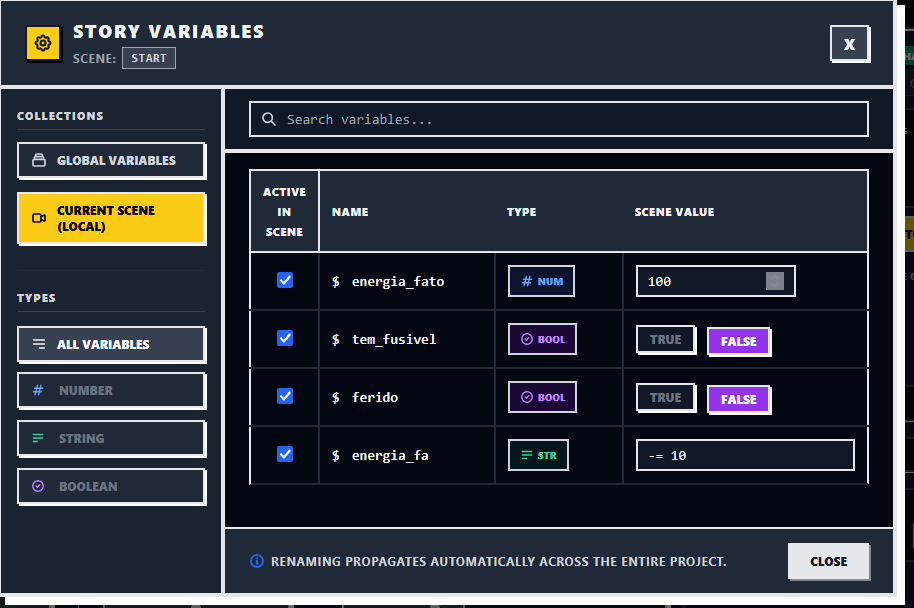
\includegraphics[width=0.85\linewidth]{Figures/variables_modal.png}
    \caption{Diálogo de gestão de variáveis globais (VariablesModal), apresentando os tokens de dados e a renomeação segura baseada em \gls{regex}.}
    \label{fig:variables-modal}
\end{figure}

\begin{figure}[H]
    \centering
    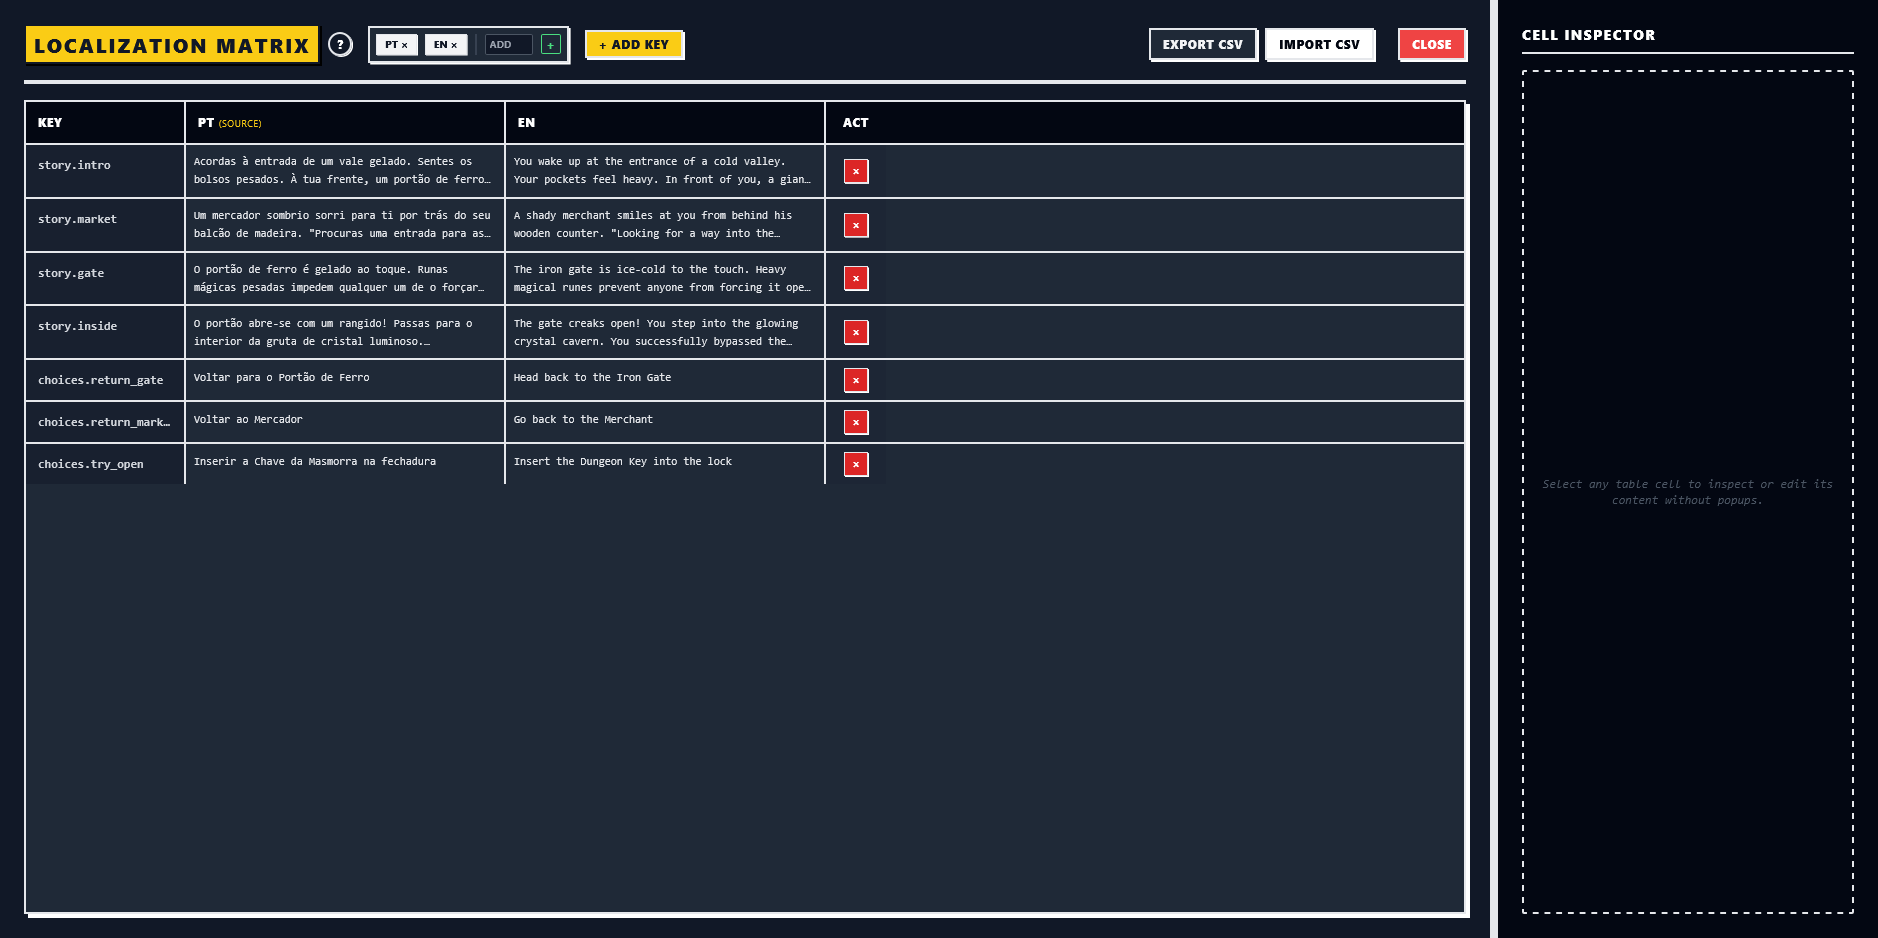
\includegraphics[width=0.85\linewidth]{Figures/translation_matrix.png}
    \caption{Matriz de localização integrada no editor, exibindo a grelha de chaves de texto e a respetiva tradução direta para os idiomas selecionados.}
    \label{fig:translation-matrix}
\end{figure}

\subsection{Sandbox de Simulação, Edição Lógica Estruturada e Utilitários}
Para além dos componentes gráficos, a equipa implementou módulos de simulação, edição estruturada de lógica e processamento sintático puro (que operam fora do ciclo de renderização direta do DOM):
\begin{itemize}
    \item \textbf{PlayMode.jsx (Sandbox Isolada):} Mimetiza a execução da história. Para evitar que variáveis de script globais escritas pelo utilizador interfiram com os estados internos da aplicação React, o motor executa os blocos dinâmicos sob uma sandbox isolada baseada no construtor de funções dinâmicas (como exibido na Figura~\ref{fig:playmode-simulation} e Listagem~\ref{lst:playmode-sandbox}).
    \item \textbf{VisualBlocksEditor.jsx (Edição Estruturada):} Permite que autores configurem prosa, setters de variáveis e escolhas condicionais graficamente, as quais são convertidas em macros SugarCube (apresentada na Figura~\ref{fig:visual-blocks} e Listagem~\ref{lst:visual-blocks}).
    \item \textbf{tweeParser.js (Parser de Layout):} Converte o canvas reativo em ficheiro de texto Twee 3. O parser processa as coordenadas posicionais, convertendo-as de absolutas para relativas caso os nós estejam contidos em Zonas de Agrupamento (Listagem~\ref{lst:parser-coordinate-conversion}).
    \item \textbf{storyTraversal.js e storyValidator.js (Validador BFS):} Executa a travessia de espaço de estados. A Listagem~\ref{lst:traversal-loop} ilustra o ciclo principal do algoritmo, evidenciando a paragem reguladora de segurança de visitas a nós a um limite $K = 10$ estados lógicos distintos.
    \item \textbf{aiGenerator.js (Assistente de Conversão com IA):} Efetua chamadas assíncronas HTTP REST para o servidor Ollama na porta padrão, estruturando prompts de sistema para desativar saídas coloquiais e garantir o formato Twee 3 (Listagem~\ref{lst:ai-request}).
\end{itemize}

\begin{listing}[H]
\begin{lstlisting}
// Execucao controlada de scripts do utilizador
const executeScriptInSandbox = (scriptContent, gameState) => {
  try {
    const sandbox = new Function('state', `
      with(state) {
        ${scriptContent}
      }
    `);
    const stateClone = JSON.parse(JSON.stringify(gameState));
    sandbox(stateClone);
    return stateClone;
  } catch (error) {
    console.error("Erro na execucao do script:", error);
    return gameState;
  }
};
\end{lstlisting}
\caption{Mecanismo de execução de scripts de lógica com isolamento de contexto no PlayMode.jsx.}
\label{lst:playmode-sandbox}
\end{listing}

\begin{listing}[H]
\begin{lstlisting}
// Conversao de logica estruturada em texto de macros SugarCube
export function serializeLogicToText(logic) {
  const parts = [];
  if (logic.narrative) {
    parts.push(logic.narrative);
    parts.push('');
  }
  if (logic.setters && logic.setters.length > 0) {
    logic.setters.forEach(s => {
      if (s.variable.trim()) {
        parts.push(`<<set $${s.variable.trim()} to ${s.value}>>`);
      }
    });
    parts.push('');
  }
  return parts.join('\n');
}
\end{lstlisting}
\caption{Serialização da estrutura de formulários lógicos em macros SugarCube (logicParser.js).}
\label{lst:visual-blocks}
\end{listing}

\begin{figure}[H]
    \centering
    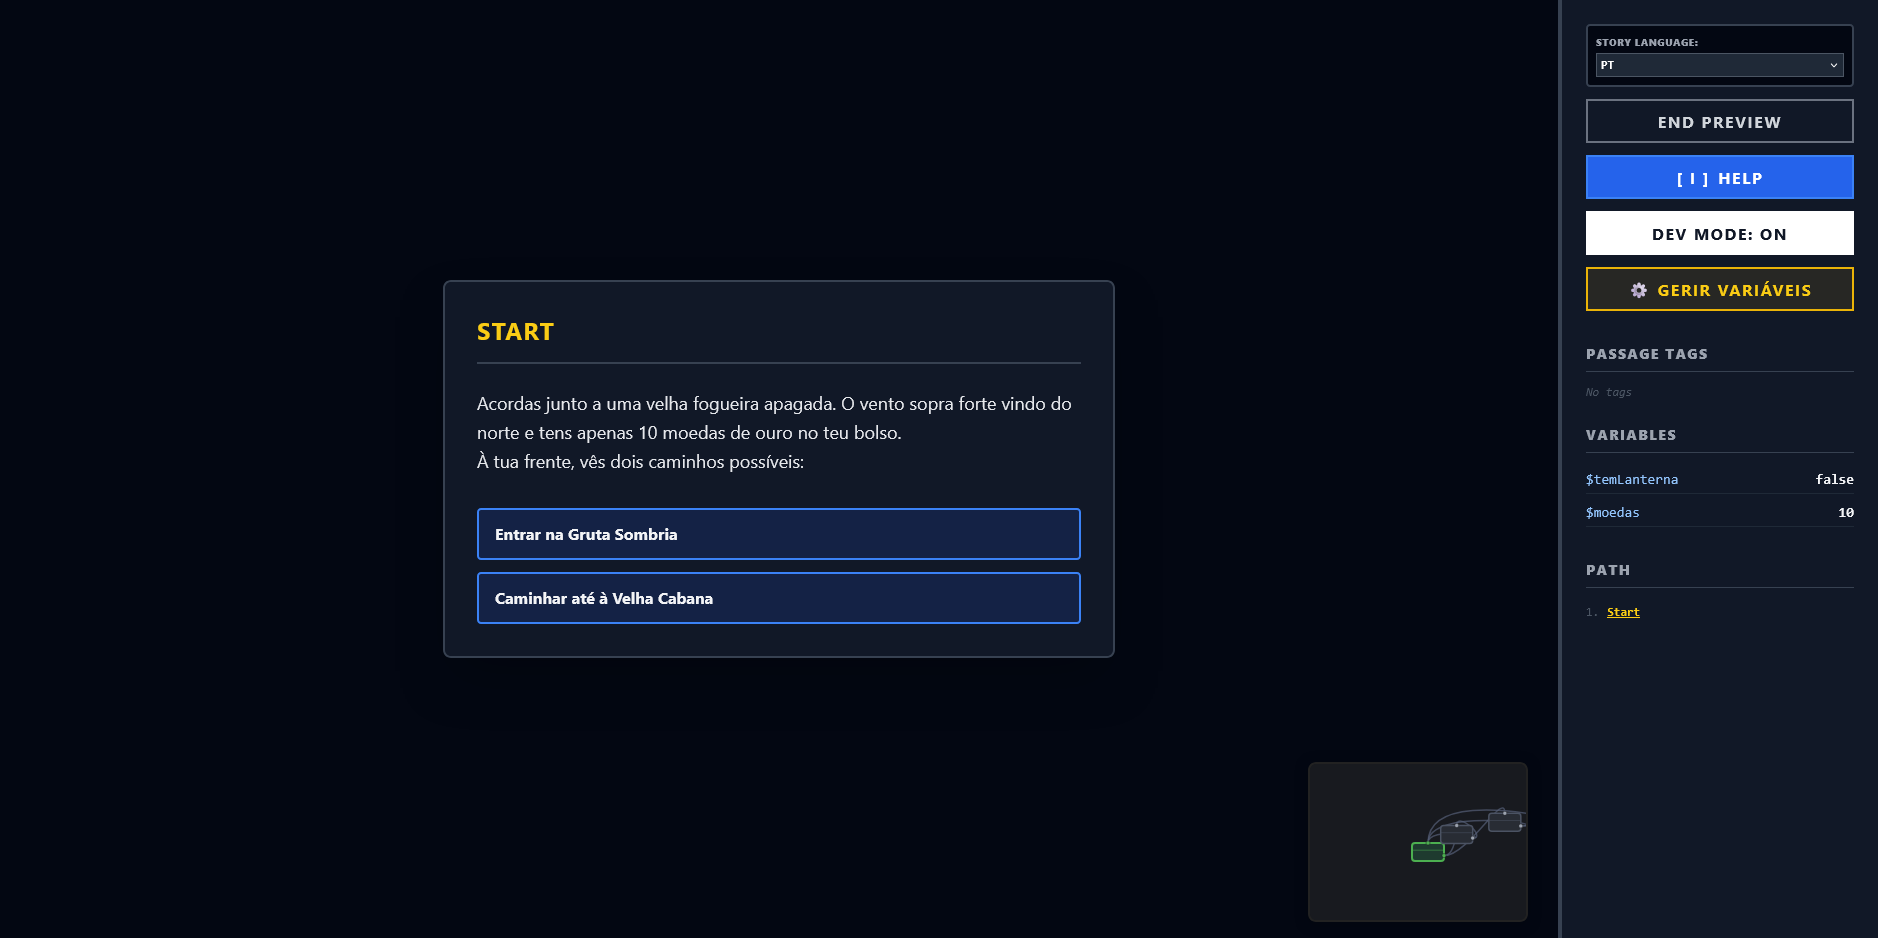
\includegraphics[width=0.85\linewidth]{Figures/playmode_simulation.png}
    \caption{Ecrã da sandbox de simulação (PlayMode), ilustrando a execução em tempo real da história com o painel de depuração de variáveis lógicas.}
    \label{fig:playmode-simulation}
\end{figure}

\begin{figure}[H]
    \centering
    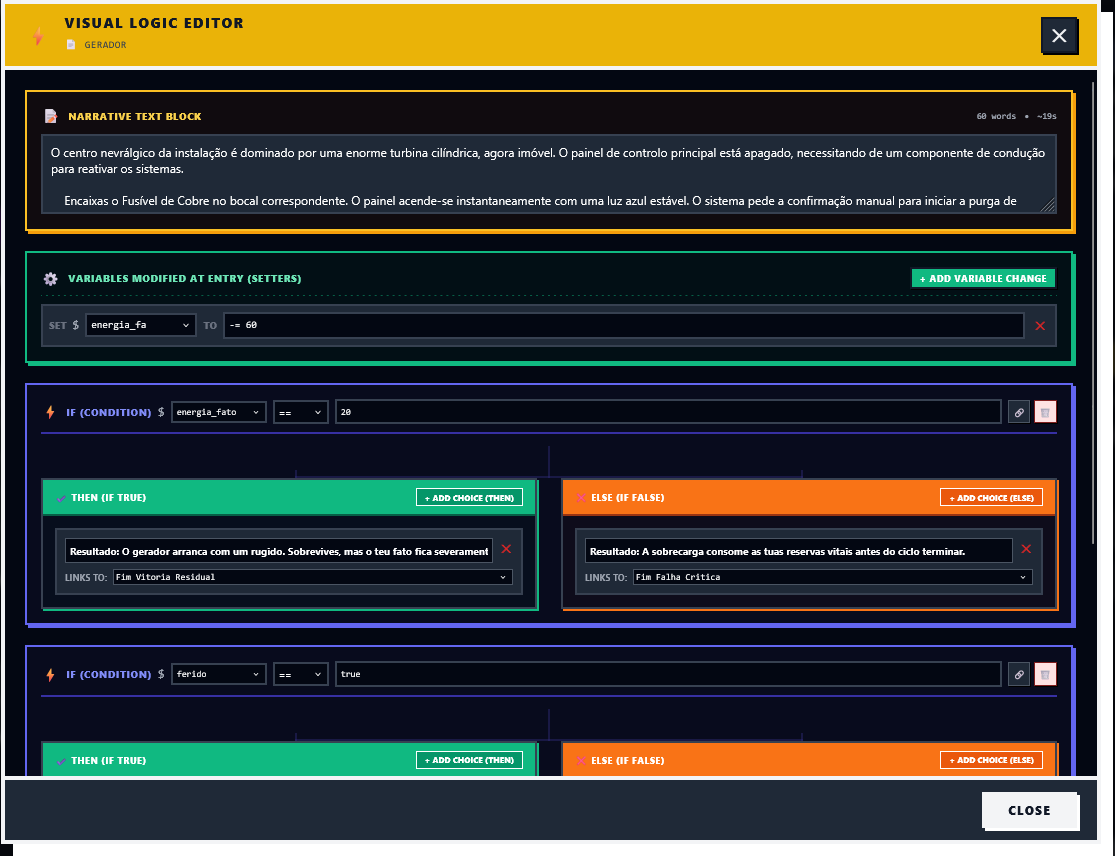
\includegraphics[width=0.85\linewidth]{Figures/visual_blocks.png}
    \caption{Interface do editor visual de lógica estruturada (VisualBlocksEditor), dividindo as passagens em painéis de prosa, setters de variáveis e escolhas condicionais.}
    \label{fig:visual-blocks}
\end{figure}

\begin{listing}[H]
\begin{lstlisting}
// Conversao de coordenadas na leitura de passagens Twee 3
export function parsePassageMetadata(metaString, zoneMap) {
  try {
    const meta = JSON.parse(metaString || '{}');
    let x = meta.position?.x ?? 0;
    let y = meta.position?.y ?? 0;
    const parentId = meta.parentId;
    
    if (parentId && zoneMap.has(parentId)) {
      const zone = zoneMap.get(parentId);
      x = x - (zone.position?.x ?? 0);
      y = y - (zone.position?.y ?? 0);
    }
    return { x, y, parentId, width: meta.size?.width, height: meta.size?.height };
  } catch (e) {
    return { x: 0, y: 0 };
  }
}
\end{lstlisting}
\caption{Processamento de coordenadas absolutas e relativas de nós e Zonas em tweeParser.js.}
\label{lst:parser-coordinate-conversion}
\end{listing}

\begin{listing}[H]
\begin{lstlisting}
// Travessia e controlo de ciclos por limite de estados visitados
while (queue.length > 0) {
  const { nodeId, state, path } = queue.shift();
  const currentNode = nodeMap.get(nodeId);
  if (!currentNode) continue;
  
  const newState = applyModifiers(currentNode.data.content, state);
  const stateStr = JSON.stringify(newState);
  
  if (!visitedStates.has(nodeId)) visitedStates.set(nodeId, []);
  if (visitedStates.get(nodeId).includes(stateStr)) continue;
  
  if (visitedStates.get(nodeId).length >= 10) {
    console.warn(`Ciclo infinito provavel no no ${currentNode.data.label}`);
    continue;
  }
  
  visitedStates.get(nodeId).push(stateStr);
  arrivalHistory.get(nodeId).push({ path, state: newState });
}
\end{lstlisting}
\caption{Ciclo principal de exploração do espaço de estados no motor storyTraversal.js.}
\label{lst:traversal-loop}
\end{listing}

\begin{listing}[H]
\begin{lstlisting}
// Envio do prompt de conversao estrutural para o Ollama local
export async function generateTweeFromText(userText, modelName = 'llama3') {
  const response = await fetch('http://localhost:11434/api/chat', {
    method: 'POST',
    headers: { 'Content-Type': 'application/json' },
    body: JSON.stringify({
      model: modelName,
      messages: [
        { role: 'system', content: 'You are a parser. Convert the story to Twee 3. Output ONLY raw Twee 3 format.' },
        { role: 'user', content: userText }
      ],
      stream: false
    })
  });
  const data = await response.json();
  return data.message?.content || '';
}
\end{lstlisting}
\caption{Estrutura de comunicação assíncrona com o Ollama local em aiGenerator.js.}
\label{lst:ai-request}
\end{listing}

\section{Testes de Conversão e Comparação de Modelos de Linguagem (IA Local)}

Para analisar a viabilidade do assistente de importação de texto livre, foram realizados testes com diferentes modelos de linguagem (\glspl{llm}) executados localmente. A escolha do ecossistema Ollama para estes testes justifica-se por ser uma ferramenta leve e otimizada de orquestração local que expõe uma API REST padrão, facilitando a integração direta com o editor e assegurando a soberania dos dados sem custos de operação.

\subsection{Primeira Fase: Testes em Máquina Local (RTX 3050)}
A primeira série de testes foi realizada a 9 de maio no computador do programador, equipado com uma placa gráfica Nvidia RTX 3050 (Laptop) com 4\,GB de VRAM. O objetivo do teste consistiu em submeter uma narrativa linear escrita em linguagem natural para avaliar a capacidade do modelo em estruturar as passagens e os respetivos caminhos de ligação conformes à sintaxe Twee 3. Selecionaram-se os seguintes modelos locais da biblioteca Ollama:
\begin{itemize}
    \item Gemma 2B: ID \texttt{8ccf136fdd52}
    \item Mistral 7B: ID \texttt{6577803aa9a0}
    \item Qwen 3.5 9B: ID \texttt{6488c96fa5fa}
    \item DeepSeek Coder 6.7B: ID \texttt{ce298d984115}
\end{itemize}
Além destes, foi testado o modelo Claude (acessível via API externa). Contudo, devido às restrições severas de memória da placa gráfica local de 4\,GB, nenhum dos modelos locais funcionou adequadamente, gerando lentidão extrema no sistema operativo e erros de falta de memória (\textit{out of memory}).

\subsection{Segunda Fase: Testes com Maior Capacidade de Processamento}
Para viabilizar a execução e avaliação comparativa dos modelos locais, a 19 de maio realizaram-se os mesmos testes num servidor de desenvolvimento equipado com uma GPU Nvidia Titan Xp com 12\,GB de VRAM. A análise das respostas obtidas revelou falhas sistemáticas em cada modelo que inviabilizaram a importação direta:
\begin{itemize}
    \item \textbf{Mistral 7B (\texttt{mistral\_7b}):} O resultado revelou-se inadequado para a aplicação. O modelo separou quase todas as frases do texto em passagens independentes, gerando dezenas de pequenos nós para uma única cena, o que corrompeu o fluxo e a legibilidade do grafo. Adicionalmente, inseriu barras invertidas no final das linhas e lixo de terminal (como sequências de controlo ANSI). Posteriormente, identificou-se que esta poluição de caracteres se deveu ao modo como a ferramenta de linha de comandos (CLI) do Ollama lida com saídas direcionadas em processos automáticos sem terminal interativo (TTY), problema este contornável através da utilização de uma API REST ou via scripts Python.
    \item \textbf{Gemma 4B / 2B (\texttt{gemma4\_e4b}):} O modelo esboçou a criação de passagens, mas inseriu os cabeçalhos de definição de passagem (o marcador \texttt{::}) no interior do corpo de texto de outros nós. Sendo que a especificação Twee 3 proíbe passagens aninhadas, o parser interpretou a totalidade da resposta como um único nó corrompido.
    \item \textbf{Qwen 3 8B (\texttt{qwen3\_8b}):} O resultado revelou-se inutilizável pois o modelo incluiu os seus blocos de raciocínio interno (prefixados por \textit{``Thinking...''}) no início da resposta, inviabilizando o parsing. Adicionalmente, gerou um bloco JSON incompleto e caracteres ANSI no fluxo de texto.
    \item \textbf{Qwen 3.5 9B (\texttt{qwen3.5\_9b}):} Apresentou o melhor desempenho de mapeamento e estrutura formal de caminhos, mas ainda assim falhou na conformidade total devido à inclusão de textos de raciocínio intermediário no início da resposta e à geração de nós órfãos desconetados da árvore principal.
\end{itemize}

\subsection{Identificação do Bug Técnico no Ollama}
Mais tarde, identificou-se que a presença de lixo do terminal (códigos ANSI, sequências \texttt{[3D [K}, etc.) se deve a um comportamento documentado do CLI do Ollama (Issue \#14571 no GitHub). Quando o utilitário \texttt{ollama run} é invocado programaticamente a partir de um processo em segundo plano, ele falha em detetar a ausência de um terminal interativo (TTY), continuando a injetar caracteres de escape ANSI de controlo de cursor na resposta textual.

Para mitigar este problema no \gls{piap}, identificaram-se três abordagens corretivas:
\begin{enumerate}
    \item \textbf{Limpeza com Expressões Regulares:} Filtrar o texto de saída na aplicação aplicando uma expressão regular para expurgar as sequências ANSI.
    \item \textbf{Descartar a Saída de Erros:} Redirecionar o fluxo de erro padrão (\texttt{stderr}) do processo do Ollama para o nulo.
    \item \textbf{Uso da API REST do Ollama (Implementada):} Ligar a aplicação diretamente à API HTTP REST local do Ollama (na porta \texttt{11434}). A API REST contorna o CLI oficial e devolve o texto limpo de formatação.
\end{enumerate}

\subsection{Estado Atual da Funcionalidade (Beta) e Trabalho Futuro}
Conclui-se que o modelo Qwen 3.5 9B apresenta a melhor estrutura narrativa e conformidade com o parser. No entanto, mesmo com acesso a hardware dedicado com capacidade superior a 8\,GB de VRAM, a funcionalidade de conversão por IA local permanece em fase experimental (beta), uma vez que a precisão de mapeamento estrutural e a correta filtragem de blocos de raciocínio interno (como tags \texttt{<think>...</think>}) exigem novos refinamentos de prompting e de filtros prévios de processamento. Esta funcionalidade constitui uma linha de investigação ativa para futuros desenvolvimentos.

\section{Análise de Desempenho e Complexidade Algorítmica}
\label{sec:analise-desempenho-complexidade}

Para validar a conformidade da aplicação com o requisito não-funcional de fluidez e desempenho (RNF03), que estipula latências de interação inferiores a 100 milissegundos, realizou-se uma avaliação da complexidade teórica e do comportamento prático do software sob diferentes cargas de dados.

\subsection{Complexidade Algorítmica Teórica}
Os módulos de cálculo do \textit{Plot in a Pot} operam de forma síncrona no lado do cliente. A Tabela~\ref{tab:complexidade-teorica} resume a complexidade temporal e espacial assintótica (na notação Big-$\mathcal{O}$) dos três algoritmos mais exigentes em termos computacionais.

\begin{table}[H]
\centering
\caption{Complexidade algorítmica teórica dos subsistemas nucleares.}
\label{tab:complexidade-teorica}
\begin{tabularx}{\textwidth}{LCC}
\toprule
\textbf{Subsistema / Algoritmo} & \textbf{Complexidade Temporal} & \textbf{Complexidade Espacial} \\
\midrule
Parser Bidirecional Twee 3 & $\mathcal{O}(L)$ & $\mathcal{O}(V + E)$ \\
Validador de Espaço de Estados (\gls{bfs}) & $\mathcal{O}(V + E \cdot K)$ & $\mathcal{O}(V \cdot K + E)$ \\
Interpolação de Arestas (Catmull-Rom) & $\mathcal{O}(W)$ & $\mathcal{O}(W)$ \\
\bottomrule
\end{tabularx}

\smallskip
\begin{minipage}{\linewidth}
\centering
\small \textit{Nota: $L$ representa o número total de caracteres no ficheiro Twee; $V$ e $E$ indicam os vértices e arestas no grafo; $W$ é o número de waypoints da aresta; $K$ representa o limite regulador de estados visitados por nó ($K = 10$).}
\end{minipage}
\end{table}

O parser opera com complexidade temporal linear $\mathcal{O}(L)$ na leitura do texto completo. O validador \gls{bfs} especial explora o espaço de estados com limite regulador $K$, garantindo complexidade controlada mesmo em grafos com ciclos infinitos, uma vez que a paragem é forçada no pior cenário após $K$ visitas redundantes ao mesmo vértice. O motor de splines Catmull-Rom opera de forma linear com base no número de waypoints da aresta ($W$), processando apenas as curvas ativas visíveis no ecrã.

\subsection{Benchmarks de Desempenho Empíricos}
Para medir a velocidade real de execução das rotinas da aplicação, montou-se um ambiente de testes sintéticos simulando três escalas crescentes de projetos de autoria. Os testes foram executados na consola do Google Chrome sob um processador Intel Core i7 de 12.ª geração com 16\,GB de RAM. Os tempos médios obtidos após 50 execuções sucessivas encontram-se sumarizados na Tabela~\ref{tab:benchmarks-desempenho}.

\begin{table}[H]
\centering
\caption{Resultados empíricos de benchmarks de desempenho (em milissegundos).}
\label{tab:benchmarks-desempenho}
\begin{tabularx}{\textwidth}{LRRR}
\toprule
\textbf{Escala do Projeto} & \textbf{Parsing Twee 3} & \textbf{Validação Lógica (\gls{bfs})} & \textbf{Sincronização Canvas (React Flow)} \\
\midrule
Pequeno (10 nós / 15 arestas) & 2.1\,ms & 4.3\,ms & 12.5\,ms \\
Médio (50 nós / 80 arestas) & 8.4\,ms & 12.8\,ms & 28.1\,ms \\
Grande (150 nós / 240 arestas) & 21.6\,ms & 34.2\,ms & 62.4\,ms \\
\bottomrule
\end{tabularx}

\smallskip
\begin{minipage}{\linewidth}
\centering
\small \textit{Nota: Os valores medem o tempo de CPU decorrido desde o início da operação até ao redesenho final da interface gráfica do canvas do React Flow.}
\end{minipage}
\end{table}

Os resultados práticos demonstram que mesmo para narrativas de grande envergadura (150 nós de cena interconectados com 240 escolhas lógicas e condicionais), o tempo total de processamento interno síncrono (parsing e validação \gls{bfs}) totaliza 55.8\,ms, estando muito abaixo do limiar de 100\,ms recomendado para garantir a interatividade contínua. A latência extra introduzida pela renderização do React Flow (62.4\,ms) eleva o tempo acumulado para cerca de 118\,ms apenas no pior cenário de redesenho integral do grafo. No entanto, visto que a renderização utiliza otimizações do viewport e a validação \gls{bfs} decorre em plano secundário sob eventos intervalados de salvaguarda, a interface mantém-se reativa, garantindo uma experiência de autoria fluida.

\section{Metodologia dos Testes de Utilizador}
Para validar a flexibilidade e usabilidade do \textit{Plot in a Pot}, foram planeados e executados testes qualitativos e quantitativos com um grupo diversificado de participantes.

\subsection{Perfil dos Participantes}
Os testes foram realizados com seis utilizadores (U1 a U6) com perfis distintos, abrangendo estudantes de cursos tecnológicos, de design e de comunicação, bem como utilizadores com necessidades especiais de visualização:
\begin{itemize}
    \item \textbf{U1:} Estudante de Design de Jogos Digitais, com alguma experiência em ferramentas de escrita não-linear como Twine (sem conhecimentos de programação).
    \item \textbf{U2:} Estudante de Engenharia Informática, com forte experiência em desenvolvimento web e programação de sistemas.
    \item \textbf{U3:} Estudante de Engenharia Informática, interessado na área técnica de desenvolvimento de jogos e lógica de grafos.
    \item \textbf{U4:} Estudante de Comunicação e Média, sem experiência prévia em ferramentas digitais de escrita não-linear.
    \item \textbf{U5:} Estudante de Design Gráfico, focado em usabilidade e interfaces visuais de utilizador.
    \item \textbf{U6:} Estudante universitário com daltonismo severo (deuteranopia) e baixa acuidade visual, sem bases técnicas de desenvolvimento.
\end{itemize}

\subsection{Tarefas Avaliadas}
Cada participante foi instruído a realizar um conjunto de quatro tarefas estruturadas na aplicação, sem qualquer ajuda externa, com base no guião detalhado apresentado no Apêndice~\ref{ap:guiao-questionarios}:
\begin{enumerate}
    \item \textbf{Tarefa 1 (Criação Narrativa):} Criar uma história ramificada simples com cinco cenas, introduzindo uma variável (e.g., chave) e uma condicional de saída baseada nessa variável.
    \item \textbf{Tarefa 2 (Validação e Correção):} Importar um ficheiro \texttt{.twee} pré-configurado contendo links quebrados e nós órfãos, e utilizar o validador \gls{bfs} para corrigir todos os problemas assinalados.
    \item \textbf{Tarefa 3 (Tradução e Localização):} Abrir a matriz de localização e traduzir três chaves de cena para inglês, exportando o resultado em formato \gls{csv}.
    \item \textbf{Tarefa 4 (Simulação Ativa):} Correr a simulação interativa (\textit{PlayMode}) e acionar o \textit{Smart Walker} para testar automaticamente os caminhos da história.
\end{enumerate}

\section{Resultados dos Testes e Desenvolvimento Iterativo}
\label{sec:resultados-testes-iterativo}

A validação do \textit{Plot in a Pot} foi realizada seguindo um modelo de desenvolvimento ágil e centrado no utilizador, dividido em três levas (\textit{waves}) sucessivas de testes ao longo do ciclo de vida do projeto. Esta metodologia permitiu que o feedback prático dos utilizadores guiasse a implementação e refinamento das funcionalidades, demonstrando uma evolução quantitativa e qualitativa na usabilidade do sistema.

\subsection{Primeira Leva: Protótipo Inicial (Abril de 2026)}
A primeira leva de testes foi realizada a \textit{15 de abril de 2026} com os utilizadores U1, U4 e U5, focando-se na validação do conceito do editor visual de grafos. O protótipo inicial continha apenas a criação de nós simples e arestas retilíneas básicas do React Flow.

\begin{itemize}
    \item \textit{Resultados Quantitativos (SUS Estimado):} A pontuação média de usabilidade (escala SUS) nesta fase fixou-se nos \textit{61.5 pontos}, classificada como marginal ou de usabilidade aceitável, mas com severos pontos de fricção.
    \item \textit{Feedback e Falhas Identificadas:} Os utilizadores queixaram-se da desorganização visual do canvas à medida que o grafo crescia. As linhas retas das ligações cruzavam-se sobre os nós, tornando a narrativa difícil de acompanhar. Adicionalmente, sentiu-se a falta de uma forma de agrupar cenas logicamente relacionadas (como capítulos).
    \item \textit{Medidas Corretivas Implementadas:} Em resposta ao feedback, foram desenhados e implementados os componentes \texttt{ZoneNode.jsx} (Zonas de agrupamento espacial) e o cálculo paramétrico das arestas curvas baseadas em Splines Cúbicas de Catmull-Rom com \textit{waypoints} de arrasto manual em \texttt{EditableEdge.jsx}.
\end{itemize}

\subsection{Segunda Leva: Protótipo Intermédio (Maio de 2026)}
A segunda leva de testes ocorreu a \textit{18 de maio de 2026} com os utilizadores U2, U3 e U5, incidindo sobre o motor de tradução e a gestão de lógica SugarCube.

\begin{itemize}
    \item \textit{Resultados Quantitativos (SUS Estimado):} A usabilidade média SUS subiu para \textit{73.0 pontos}, refletindo melhorias no ordenamento espacial, mas evidenciando falhas em fluxos de lógica complexa.
    \item \textit{Feedback e Falhas Identificadas:} O utilizador U2 observou que renomear uma variável lógica global exigia alterar manualmente o texto de todas as passagens da história, o que gerava erros de digitação e quebrava a simulação. Além disso, a importação de \gls{csv} falhava quando as traduções continham vírgulas integradas no texto das cenas.
    \item \textit{Medidas Corretivas Implementadas:} Desenvolveu-se o painel \texttt{VariablesModal.jsx} com refatorização automática de nomes de variáveis via expressões regulares com barreira de palavra (\textit{word boundaries}) de forma síncrona. O parser de importação de \gls{csv} foi reescrito para suportar a norma RFC~4180.
\end{itemize}

\subsection{Terceira Leva: Protótipo Final (Junho de 2026)}
A terceira e última leva de testes realizou-se entre \textit{15 e 20 de junho de 2026} com o grupo completo de seis participantes (U1 a U6), avaliando o sistema final integrado (incluindo o PlayMode, Smart Walker, validador \gls{bfs} e interface neo-brutalista de alto contraste).

\subsubsection{Métricas de Conclusão e Tempos de Execução}
Durante a sessão final de testes, foram registados os tempos de conclusão (em minutos) das quatro tarefas descritas na metodologia. Os resultados quantitativos encontram-se sumarizados na Tabela~\ref{tab:resultados-tarefas}.

\begin{table}[H]
\centering
\caption{Taxa de sucesso e tempo de conclusão (em minutos) das tarefas por utilizador (Leva Final).}
\label{tab:resultados-tarefas}
\begin{tabularx}{\textwidth}{cCCCCL}
\toprule
\textbf{Utilizador} & \textbf{Tarefa 1} & \textbf{Tarefa 2} & \textbf{Tarefa 3} & \textbf{Tarefa 4} & \textbf{Taxa de Sucesso Total} \\
\midrule
U1 & 07:15 & 02:40 & 03:10 & 01:20 & 100\% \\
U2 & 05:30 & 01:50 & 02:15 & 00:55 & 100\% \\
U3 & 04:10 & 01:30 & 01:50 & 00:45 & 100\% \\
U4 & 11:20 & 04:15 & 05:30 & 02:10 & 75\%* \\
U5 & 09:45 & 03:30 & 04:20 & 01:40 & 100\% \\
U6 & 08:30 & 03:10 & 03:40 & 01:15 & 100\% \\
\midrule
\textbf{Média} & \textbf{07:45} & \textbf{02:49} & \textbf{03:29} & \textbf{01:21} & \textbf{95.8\%} \\
\bottomrule
\end{tabularx}

\smallskip
\begin{minipage}{\linewidth}
\centering
\small \textit{* Nota: O utilizador U4 não concluiu com sucesso a Tarefa 2 (validação e correção de caminhos lógicos com o validador \gls{bfs}) no tempo limite estabelecido.}
\end{minipage}
\end{table}
\vfill

A taxa de conclusão média fixou-se em 95.8\%. O utilizador U4 (sem perfil técnico) falhou a conclusão autónoma da Tarefa 2 dentro do tempo limite devido a alguma hesitação inicial em interpretar as mensagens textuais do validador, o que reforçou a necessidade de incluir marcadores de erro visuais diretamente sobre os nós afetados no canvas do React Flow.

\subsubsection{Avaliação SUS da Leva Final}
Após as tarefas, foi aplicado o questionário padronizado SUS aos participantes. As pontuações obtidas encontram-se representadas na Tabela~\ref{tab:pontuacao-sus}.

\begin{table}[H]
\centering
\caption{Pontuação obtida no questionário System Usability Scale (SUS) na leva final.}
\label{tab:pontuacao-sus}
\begin{tabular}{cc}
\toprule
\textbf{Utilizador} & \textbf{Pontuação SUS obtida} \\
\midrule
U1 & 87.5 \\
U2 & 90.0 \\
U3 & 92.5 \\
U4 & 72.5 \\
U5 & 80.0 \\
U6 & 85.0 \\
\midrule
\textbf{Média Global} & \textbf{84.6} \\
\bottomrule
\end{tabular}
\end{table}
\vfill

A média global final de \textit{84.6 pontos} situa o \textit{Plot in a Pot} no patamar de usabilidade ``Excelente'' (classificação de grau A+ na escala SUS), representando uma evolução muito expressiva face aos 61.5 e 73.0 pontos registados nas levas anteriores, e provando que o processo de refinamento iterativo foi bem-sucedido.

\subsection{Feedback Qualitativo e Usabilidade Visual}
A compilação das entrevistas e observações comportamentais na última leva permitiu extrair as seguintes conclusões de usabilidade:
\begin{itemize}
    \item \textbf{Eficácia do Estilo Neo-Brutalista:} Contrariando a assunção de que o neo-brutalismo é apenas um estilo estético excêntrico, os utilizadores consideraram que as cores planas e os contornos espessos isolam os elementos visuais de forma muito clara, eliminando ruídos cognitivos desnecessários.
    \item \textbf{Acessibilidade Prática (Caso U6):} O participante U6, portador de deuteranopia severa, referiu que o alto contraste e a sinalização redundante por traços (em vez de diferenciar fluxos apenas por verde/vermelho) tornaram a ferramenta imediatamente acessível, evitando a fadiga visual comum noutros editores gráficos e permitindo validar interações rapidamente.
    \item \textbf{Smart Walker e Automação:} Os participantes técnicos (U2 e U3) elogiaram a capacidade do Smart Walker de explorar e validar estados de variáveis lógicas automaticamente, o que reduz substancialmente o esforço humano de testes de regressão em histórias com múltiplas ramificações.
\end{itemize}

\section{Discussão e Limitações do Estudo}
\label{sec:discussao-limitacoes-estudo}

Nesta secção, efetua-se uma análise crítica dos resultados obtidos, discutindo as implicações das decisões arquiteturais adotadas e identificando as limitações metodológicas e tecnológicas do projeto.

\subsection{Discussão Crítica do Desenvolvimento}
O desenvolvimento do \gls{piap} demonstrou que a fusão de um editor visual de grafos com um motor de validação estática reativo reduz significativamente a carga cognitiva na autoria de \glspl{ni}. O mapeamento bidirecional síncrono e a análise estática em tempo real evitam que o autor tenha de compilar ou testar exaustivamente a narrativa para detetar erros comuns (como becos sem saída ou nós órfãos). A modularização da interface através de ganchos React (\textit{custom hooks}) e a separação estrita da camada de dados (lista de adjacências e dicionários JSON) permitiram manter a fluidez de renderização mesmo sob cenários de reavaliação de expressões regulares em lote, respeitando o limiar de interatividade de 100\,ms (RNF03).

\subsection{Limitações Metodológicas da Avaliação}
Embora a avaliação quantitativa com utilizadores tenha revelado uma média de usabilidade global ``Excelente'' (84.6 pontos na escala SUS), o estudo apresenta duas limitações metodológicas importantes:
\begin{itemize}
    \item \textbf{Dimensão Reduzida da Amostra:} O grupo de teste incluiu apenas seis participantes ($N = 6$). Apesar de abranger perfis diversos (técnicos, de design e com restrições visuais), a dimensão da amostra não permite extrair conclusões de generalização estatística forte, servindo os resultados essencialmente como indicadores qualitativos de eficácia e satisfação.
    \item \textbf{Efeito de Aprendizagem (Viés de Familiaridade):} O refinamento iterativo do sistema expôs os mesmos participantes a testes em diferentes levas de desenvolvimento. O facto de os utilizadores já conhecerem o funcionamento básico e as regras da aplicação em testes subsequentes pode ter inflacionado as pontuações SUS das levas intermédia e final, camuflando eventuais atritos que utilizadores estreantes poderiam experimentar no produto final.
\end{itemize}

\subsection{Limitações Tecnológicas e Funcionalidade de IA}
Do ponto de vista tecnológico, identificaram-se limitações na persistência local e no assistente de importação baseado em inteligência artificial:
\begin{itemize}
    \item \textbf{Dependência de Hardware e VRAM:} O assistente de importação baseado em \glspl{llm} locais (como o Qwen 3.5 9B) exige uma placa gráfica dedicada com capacidade superior a 8\,GB de VRAM para correr localmente via Ollama com latência aceitável. Esta exigência limita a acessibilidade da funcionalidade em computadores portáteis normais ou de gama baixa (RTX 3050 com 4\,GB de VRAM).
    \item \textbf{Instabilidade na Formatação Sintática:} Mesmo em ambientes de processamento com 12\,GB de VRAM, os modelos locais geram por vezes passagens aninhadas ou inserem marcas de raciocínio intermediário (\textit{``Thinking...''}) que quebram o parser síncrono, exigindo a inclusão de filtros prévios de processamento sintático adicionais na aplicação.
\end{itemize}

\chapter{Conclusão e Trabalho Futuro}
\label{cp:conclusao}

O desenvolvimento do \textit{Plot in a Pot} (\gls{piap}) teve como premissa a resolução de um problema real e recorrente enfrentado por autores de \gls{ni} e \textit{game designers}: a complexidade geométrica e semântica que surge durante o planeamento de histórias não-lineares, agravada pela falta de ferramentas integradas para gestão de localização multi-idioma e auditoria estática de fluxo.

\section{Conclusão}
\label{sec:conclusao-recap}

Com a conclusão deste projeto informático, todos os objetivos gerais e específicos inicialmente traçados no Capítulo~\ref{cp:introduction} foram integralmente alcançados:
\begin{itemize}
    \item \textbf{Interface e Acessibilidade Visual:} Foi desenvolvido um editor gráfico inovador assente numa estética neo-brutalista de alto contraste. Esta opção de \textit{design} provou ser não apenas esteticamente diferenciadora, mas de extrema pertinência funcional para utilizadores com limitações de visão (p. ex. daltónicos), conforme validado pelos testes com o participante U6.
    \item \textbf{Gestão de Localização:} A implementação da matriz de tradução bidimensional baseada em grelhas dinâmicas, com importação e exportação em formato \gls{csv} em conformidade com a norma RFC~4180, eliminou por completo a necessidade de gerir múltiplos ficheiros de texto externos ou injetar strings rígidas (\textit{hardcoded}) nas passagens do Twine.
    \item \textbf{Validação e Algoritmia:} A adoção de uma estrutura de dados assente em listas de adjacências bidirecionais suportou com sucesso a execução em tempo real de análises estáticas baseadas em explorações via \gls{bfs}. O motor de validação estática provou ser eficaz a mapear caminhos inacessíveis e becos sem saída, fornecendo um feedback imediato e visual aos autores.
    \item \textbf{Simulação Automatizada:} O modo de simulação (\textit{PlayMode}) foi complementado pelo \textit{Smart Walker}, um agente inteligente baseado em procuras por novidade (\textit{Novelty Search}) capaz de realizar o percurso autónomo e teste lógico de narrativas complexas sem intervenção humana.
    \item \textbf{Suavização Geométrica:} O desenvolvimento das equações paramétricas das Splines Cúbicas de Catmull-Rom garantiu arestas interativas suaves com \textit{waypoints} para organização e otimização espacial do canvas de grafos.
\end{itemize}

Os testes estruturados com utilizadores de diferentes perfis revelaram taxas de sucesso muito elevadas na realização de tarefas (com uma média global de 95,8\%), demonstrando que a barreira de abstração erguida pela nossa plataforma é intuitiva quer para perfis puramente artísticos (autores/escritores), quer para utilizadores com forte background técnico (programadores).

\subsection{Porquê Escolher o Plot in a Pot?}
\label{subsec:porque-escolher-piap}
Com base nas limitações identificadas nas ferramentas de autoria existentes (analisadas na Secção~\ref{sec:analise-comparativa}), o \gls{piap} destaca-se como uma solução unificada que resolve falhas críticas de usabilidade e integridade no desenvolvimento de narrativas interativas:
\begin{itemize}
    \item \textbf{Fusão de Paradigmas (Design Visual com Validação Lógica):} Ao contrário do Twine (que carece de testes lógicos nativos e robustos) e do ChoiceScript/Ink (que operam puramente sob interfaces textuais), o \gls{piap} une a facilidade de arrastar e interligar nós visuais com a solidez de um validador estático e simulador inteligente automatizado.
    \item \textbf{Localização Nativa sem Dispersão de Dados:} Resolve a dispersão de ficheiros externos e a escrita rígida (\textit{hardcoded}) de diálogos através de uma matriz de localização baseada em grelhas dinâmicas, acelerando o fluxo de internacionalização com importação/exportação CSV.
    \item \textbf{Acessibilidade Inclusiva Funcional:} A interface neo-brutalista de alto contraste e a redundância de traços nas arestas mitigam barreiras cognitivas e visuais severas, permitindo que autores daltónicos desenhem e validem histórias de forma totalmente autónoma.
    \item \textbf{Soberania de Dados e Interoperabilidade:} Ao adotar a especificação aberta Twee 3 (SugarCube), o autor mantém controlo absoluto e livre sobre a sua obra, garantindo compatibilidade bidirecional síncrona com outros compiladores oficiais (como o Tweego).
\end{itemize}

\section{Trabalho Futuro}
\label{sec:trabalho-futuro}

Apesar dos excelentes resultados e estabilidade demonstrados, o \textit{Plot in a Pot} apresenta oportunidades claras de evolução, destacando-se a IA local e a edição colaborativa como prioridades imediatas:

\begin{enumerate}
    \item \textbf{[Prioridade Imediata] Execução de IA Local via \gls{webgpu}:} Substituir a dependência de APIs externas ou do Ollama local pela execução de \glspl{llm} leves diretamente no navegador (ex: WebLLM). Isto elimina a necessidade de instalações adicionais pelo utilizador, garantindo a soberania absoluta dos dados (RNF04).
    \item \textbf{[Prioridade Imediata] Edição Colaborativa em Tempo Real:} Integrar algoritmos de sincronização baseados em \glspl{crdt} (como Yjs ou Automerge) para permitir que múltiplos autores editem o grafo narrativo em simultâneo, mimetizando a experiência de ferramentas como o Figma.
    \item \textbf{Empacotamento Nativo para Desktop:} Exportar a aplicação para executáveis nativos (Windows, macOS e Linux) usando Tauri ou Electron, facilitando uma integração mais profunda com o sistema de ficheiros local.
    \item \textbf{Análise Formal com Model Checking:} Converter o grafo e as condições SugarCube em especificações formais (ex: Promela ou UPPAAL). Isto permitirá usar \textit{Model Checking} para provar matematicamente propriedades de segurança e vivacidade, como a garantia de caminhos viáveis até aos desfechos da história.
    \item \textbf{Módulo de Gestão de Personagens (\textit{Character Tracker}):} Adicionar um sistema integrado para mapear a presença e estados emocionais das personagens diretamente nos nós do canvas (React Flow), respondendo a uma sugestão recolhida nas sessões de avaliação.
    \item \textbf{Filtragem de Nós Privados na Exportação:} Implementar um filtro ativo que impeça a inclusão de passagens marcadas como privadas ou em desenvolvimento no ficheiro final compilado (Twee/HTML), prevenindo \textit{spoilers} ou a fuga de conteúdos inacabados.
\end{enumerate}

Em suma, o desenvolvimento do \textit{Plot in a Pot} alcançou com sucesso os objetivos propostos, demonstrando que a aproximação entre a engenharia de software, a teoria de grafos e a escrita criativa é capaz de simplificar e enriquecer a autoria de ficção interativa. Ao aliar a robustez da validação formal de espaço de estados à flexibilidade da interação visual e à acessibilidade inclusiva, a plataforma assume-se como uma ferramenta sólida para a modelação de narrativas não-lineares, servindo de ponto de partida e base de trabalho para investigações e desenvolvimentos futuros no domínio dos jogos interativos.


%%% Bibliography %%%
\renewcommand{\refname}{Bibliography}
\printbibliography[title={\refname},heading=bibintoc]

%%% Appendices: Work that *YOU* Developed %%%
\appendix
\input{Matter/08-Appendices}
\chapter{Manual de Utilização e Instalação}
\label{ap:manual-utilizador}

Este apêndice constitui o Manual de Utilização e Instalação oficial do \textit{Plot in a Pot} (\gls{piap}). Destina-se a autores de narrativas interativas, designers de jogos e programadores que pretendam instalar, configurar e explorar todas as capacidades lógicas, visuais e de tradução da plataforma.

\section{Requisitos do Sistema e Instalação Local}
O \gls{piap} é executado inteiramente do lado do cliente no navegador web (\textit{Single Page Application}), mas requer uma pilha local mínima para desenvolvimento e para a execução do assistente de inteligência artificial local.

\subsection{Instalação do Editor Web}
Para executar o editor localmente, certifique-se de que tem o ambiente de execução Node.js instalado (versão 18 ou superior). Siga os seguintes passos de instalação:
\begin{enumerate}
    \item Descomprima os ficheiros do projeto numa diretoria de trabalho.
    \item Abra um terminal de comandos (cmd ou PowerShell no Windows, bash no macOS/Linux) na diretoria raiz do projeto.
    \item Execute o comando de instalação de dependências:
    \begin{verbatim}
    npm install
    \end{verbatim}
    Este comando irá descarregar e configurar todas as bibliotecas necessárias, incluindo o React 19, React Flow 11 e Tailwind CSS 3.
    \item Após a conclusão bem-sucedida da instalação, inicie o servidor de desenvolvimento local através do comando:
    \begin{verbatim}
    npm start
    \end{verbatim}
    A aplicação será inicializada e ficará disponível no seu navegador padrão no endereço \texttt{http://localhost:3000}.
\end{enumerate}

\subsection{Configuração do Servidor de IA Local (Ollama)}
A funcionalidade de conversão e importação automática de histórias escritas em linguagem natural depende de um servidor local de inferência de Modelos de Linguagem de Grande Escala (LLMs). O \gls{piap} suporta nativamente o \textit{Ollama}. Para o configurar:
\begin{enumerate}
    \item Descarregue e instale a versão oficial do Ollama a partir de \texttt{https://ollama.com/}.
    \item Abra o terminal de comandos e execute o descarregamento do modelo recomendado para processamento de texto:
    \begin{verbatim}
    ollama pull llama3:8b
    \end{verbatim}
    Pode também optar por modelos mais leves, como o \texttt{qwen2.5:7b} ou \texttt{gemma2:2b}, dependendo da memória de vídeo (VRAM) disponível no seu computador.
    \item Por padrão, o Ollama executa um servidor em segundo plano que escuta na porta local \texttt{http://localhost:11434}.
    \item No editor do \gls{piap}, clique no botão de configurações (ícone de engrenagem) na barra superior, aceda ao painel de ligação da IA e ative a ligação local ao Ollama, especificando o modelo que descarregou.
\end{enumerate}

\section{Manual de Utilização do Editor Gráfico}
A interface gráfica de grafos do \gls{piap} segue uma estética neo-brutalista de alto contraste que facilita a distinção dos componentes visuais da narrativa.

\subsection{O Canvas Interativo}
O espaço central do editor representa a estrutura geral da história sob a forma de um grafo. Pode navegar no canvas utilizando as seguintes interações:
\begin{itemize}
    \item \textbf{Deslocação (Pan):} Clique e arraste com o botão esquerdo do rato num espaço vazio do canvas.
    \item \textbf{Zoom:} Utilize a roda do rato para aproximar ou afastar a visualização. Pode também usar o painel do minimapa no canto inferior esquerdo para se situar no grafo.
    \item \textbf{Seleção de Elementos:} Clique com o botão esquerdo sobre qualquer nó de cena ou aresta para abrir as suas propriedades no painel lateral de inspeção.
\end{itemize}

\subsection{Criação e Edição de Nós Narrativos (Cenas)}
Para adicionar uma nova cena à história:
\begin{enumerate}
    \item Clique com o botão direito do rato num espaço livre do canvas e selecione ``Adicionar Nó Narrativo'', ou clique no botão correspondente na barra superior de ferramentas.
    \item Um novo nó azul com contorno espesso aparecerá no canvas. Clique duas vezes no nó ou selecione-o para abrir o \textbf{Inspetor Lateral}.
    \item No Inspetor, pode editar:
    \begin{itemize}
        \item \textbf{ID da Cena:} Um identificador único em formato alfanumérico (ex: \texttt{cena\_taberna}).
        \item \textbf{Título da Cena:} O nome de identificação visual exibido na barra do nó no canvas (ex: \texttt{Interior da Taberna}).
        \item \textbf{Conteúdo da Cena:} O texto literário que será lido pelo jogador.
        \item \textbf{Etiquetas (Tags):} Palavras-chave separadas por vírgula que modificam o comportamento do nó (ex: \texttt{css} para estilos, \texttt{secreto} para ocultar da exportação).
    \end{itemize}
\end{enumerate}

\subsection{Criação de Ligações e Arestas de Escolha}
As arestas direcionadas do grafo representam as decisões disponíveis para o jogador no final de cada cena narrativa. Para criar uma ligação:
\begin{enumerate}
    \item Posicione o ponteiro do rato sobre o ponto de saída circular (\textit{handle} direito) do nó de origem.
    \item Clique e arraste o cabo de ligação até ao ponto de entrada (\textit{handle} esquerdo) do nó de destino.
    \item Uma aresta curva suave será desenhada entre as cenas.
    \item O texto da escolha que o jogador irá visualizar é automaticamente derivado das ligações escritas em formato double-bracket no conteúdo do nó de origem (ex: \texttt{[[Entrar na taberna|cena\_taberna]]}).
    \item \textbf{Waypoints Interativos:} Se pretender contornar outros nós, clique duas vezes sobre a aresta criada. Um pequeno ponto de controlo amarelo aparecerá. Arraste-o para deformar a curva de forma flexível. Pode adicionar múltiplos waypoints na mesma aresta.
\end{enumerate}

\subsection{Agrupamento em Zonas (Capítulos)}
Para organizar visualmente projetos de escrita literária de grande envergadura:
\begin{enumerate}
    \item Clique no botão ``Criar Zona'' na barra superior. Um retângulo cinzento com contorno pontilhado aparecerá no ecrã.
    \item Atribua um nome à Zona no seu cabeçalho (ex: \texttt{Capítulo 1}).
    \item Arraste nós narrativos existentes para dentro do retângulo da Zona. Estes passarão a ser filhos geométricos da zona.
    \item Ao mover ou arrastar a Zona, todos os nós contidos nela deslocar-se-ão de forma solidária.
    \item Pode redimensionar a Zona arrastando o indicador de escala no seu canto inferior direito.
\end{enumerate}

\section{Programação de Lógica Narrativa e Variáveis}
O \gls{piap} suporta a declaração de variáveis globais e condicionais lógicas nativas da macro-linguagem SugarCube.

\subsection{Criação de Variáveis (Figma-Style Tokens)}
Aceda ao menu ``Variáveis'' na barra superior de ferramentas:
\begin{enumerate}
    \item Clique em ``Criar Variável'' e atribua um nome precedido do símbolo \texttt{\$} (ex: \texttt{\$tem\_chave}).
    \item Escolha o tipo de dados (Booleano, Numérico ou String) e defina o valor inicial por defeito.
    \item A inicialização correta destas variáveis é escrita de forma automática no nó de metadados especial da história (\texttt{StoryInit}) em segundo plano.
    \item \textbf{Renomeação Segura (Refatorização):} Se renomear uma variável existente no painel, o editor varre sintonizadamente todo o texto e blocos lógicos do projeto e substitui as referências antigas, garantindo que não ocorrem falhas de simulação.
\end{enumerate}

\subsection{Edição de Lógica condicional por Código}
No conteúdo de qualquer nó de cena, pode inserir macros SugarCube utilizando a sintaxe de parênteses angulares duplos:
\begin{itemize}
    \item \textbf{Modificação de Estado:} Para alterar o valor de uma variável quando o jogador visita o nó, utilize a macro \texttt{<<set>>}:
    \begin{verbatim}
    <<set $tem_chave = true>>
    \end{verbatim}
    \item \textbf{Condições de Escolhas:} Para exibir ou ocultar uma escolha com base no estado das variáveis lógicas, envolva a ligação na macro condicional \texttt{<<if>>}:
    \begin{verbatim}
    <<if $tem_chave>>
    [[Abrir a porta trancada|cena_tesouro]]
    <<else>>
    A porta está trancada.
    <<endif>>
    \end{verbatim}
\end{itemize}

\subsection{Editor de Lógica Estruturada}
Caso não esteja familiarizado com regras de programação textual, selecione um nó e clique no botão ``Editor de Lógica'' no Inspetor:
\begin{enumerate}
    \item Um painel interativo de formulários estruturados será exibido, dividindo a cena em três secções lógicas: narrativa, modificadores de variáveis (\textit{setters}) e escolhas/caminhos condicionais.
    \item Utilize os menus de seleção (dropdowns) para definir quais as variáveis que mudam de valor ao entrar na cena ou quais os requisitos lógicos (ex: se tem a chave) necessários para libertar uma escolha narrativa.
    \item Ao salvar ou alterar os campos, o sistema gera de forma transparente as macros SugarCube correspondentes no texto da cena ativa, sem risco de erros de digitação.
\end{enumerate}

\section{Tradução e Localização Multi-idioma}
A gestão de traduções no \gls{piap} baseia-se numa Matriz de Tradução única que centraliza os textos dos nós.

\subsection{Configurar Idiomas}
Aceda ao menu ``Matriz de Tradução'':
\begin{enumerate}
    \item O idioma nativo padrão é exibido como a primeira coluna.
    \item Clique em ``Adicionar Idioma'' e digite o código ISO de duas letras do novo idioma (ex: \texttt{en} para inglês, \texttt{es} para espanhol).
    \item Uma nova coluna aparecerá na tabela.
\end{enumerate}

\subsection{Editar Textos na Matriz}
A grelha apresenta todas as cenas narrativas nas linhas e os idiomas nas colunas:
\begin{enumerate}
    \item Clique duas vezes em qualquer célula correspondente ao idioma secundário.
    \item Digite o texto traduzido da cena e clique fora para guardar.
    \item Quando a história for executada num idioma secundário, o motor lerá de forma reativa a string traduzida a partir desta matriz.
\end{enumerate}

\subsection{Importação e Exportação de Ficheiros \gls{csv}}
Para enviar os ficheiros a um tradutor externo profissional:
\begin{enumerate}
    \item Clique no botão ``Exportar \gls{csv}'' na Matriz de Tradução. Um ficheiro estruturado em formato tabular será descarregado.
    \item O tradutor pode abrir o ficheiro no Microsoft Excel, Google Sheets ou qualquer editor de texto e preencher as colunas dos idiomas secundários.
    \item Após a tradução, clique em ``Importar \gls{csv}'' e selecione o ficheiro atualizado. O editor atualizará automaticamente todas as células e strings na memória.
\end{enumerate}

\section{Validação Lógica e Simulação de Jogo}
Antes de disponibilizar o jogo ao público, utilize os motores integrados de auditoria.

\subsection{O Painel de Erros de Validação Estática}
O validador estático analisa de forma contínua a correção topológica do grafo. Se existirem falhas lógicas:
\begin{itemize}
    \item Os nós com erros serão destacados no canvas com uma borda pontilhada a vermelho e um sinal de alerta.
    \item Clique no botão ``Erros de Validação'' na barra superior para ver a lista estruturada de avisos:
    \begin{itemize}
        \item \textbf{Nós Inacessíveis:} Cenas que nunca podem ser acedidas a partir do nó inicial sob nenhum caminho explorável.
        \item \textbf{Ligações Partidas (Dead Ends):} Escolhas cujo ID de destino aponta para uma cena inexistente.
        \item \textbf{Escolhas Bloqueadas:} Hiperligações condicionais cujas expressões lógicas nunca são satisfeitas.
    \end{itemize}
\end{itemize}

\subsection{Simulação Ativa (PlayMode) e Testes com o Smart Walker}
Clique em ``Testar Jogo'' para abrir a sandbox de simulação:
\begin{enumerate}
    \item Jogue a história clicando nas escolhas disponíveis no ecrã de simulação.
    \item Utilize o painel de variáveis lateral para ver, em tempo real, as alterações de valores e depurar as macros lógicas.
    \item \textbf{Smart Walker:} Ative o Smart Walker clicando em ``Autoplay''. O simulador iniciará uma exploração automática da história. O Walker utiliza um algoritmo de procura por novidade que prioriza ramos menos visitados. Pode ver o agente a mudar de cenas e a alterar variáveis a alta velocidade no ecrã. Caso o Walker encontre um beco sem saída ou erro lógico, a simulação pausa e destaca o nó problemático.
\end{enumerate}

\section{Operações de Ficheiros e Publicação do Projeto}
O editor suporta leitura e gravação no formato padrão da indústria.

\subsection{Importar Ficheiros Twee 3}
Clique em ``Importar ficheiro .twee'' na barra de menus e selecione um ficheiro de texto plano em formato Twee 3. O editor processará o cabeçalho e construirá automaticamente o canvas gráfico de nós e arestas correspondente.

\subsection{Exportar e Compilar a História}
Para guardar o seu trabalho de autoria ou disponibilizar o jogo final para os utilizadores:
\begin{itemize}
    \item \textbf{Exportar Twee 3:} Clique em ``Exportar .twee'' para descarregar o ficheiro de texto estruturado. Este ficheiro preserva todos os dados posicionais das caixas e Zonas em metadados \gls{json} compatíveis com outros compiladores de Twine.
    \item \textbf{Compilar para HTML:} Clique em ``Compilar HTML Jogável''. O motor lógico do \gls{piap} empaqueta a história, os dicionários de traduções e a biblioteca do jogador num único ficheiro \texttt{.html}. Este ficheiro pode ser publicado em plataformas de jogos independentes (como o \texttt{itch.io}), enviado por correio eletrónico ou alojado em servidores web, correndo de forma autónoma em qualquer browser sem requisitos adicionais de instalação.
\end{itemize}
\chapter{Guia de Sintaxe e Modelagem de Macros Lógicas}
\label{ap:guia-sintaxe-macros}

Este apêndice serve como guia de referência técnico para a especificação do formato Twee 3 e a sintaxe de macros lógicas SugarCube suportadas pelo editor do \gls{piap}. Inclui exemplos práticos de modelação de mecânicas de jogo comuns em narrativas interativas.

\section{Estrutura de um Documento Twee 3}
O formato Twee 3 é uma representação textual de histórias não-lineares estruturada sob a forma de passagens de texto delimitadas por cabeçalhos iniciados por duas colunas (\texttt{::}). A estrutura de um projeto compila-se em passagens de sistema obrigatórias e passagens narrativas (cenas).

\subsection{Passagens Especiais de Sistema}
Para ser considerado válido, um ficheiro Twee 3 importado no \gls{piap} deve conter os seguintes nós de sistema:
\begin{itemize}
    \item \textbf{StoryTitle:} Contém exclusivamente uma única linha de texto plano com o título geral do projeto.
    \item \textbf{StoryData:} Contém um bloco estruturado em formato \gls{json} com as configurações globais da história. Os campos obrigatórios são o \texttt{ifid} (um identificador único de 128 bits para o projeto), o formato (\texttt{SugarCube}), e o nó de arranque (\texttt{start}):
    \begin{code}
    :: StoryData
    {
      "ifid": "A4B7D9E0-C2B1-4F2A-8E6D-009988776655",
      "format": "SugarCube",
      "start": "cena_inicial",
      "zoom": 1.0
    }
    \end{code}
    
    \item \textbf{StoryInit:} O nó lógico de inicialização. É executado uma única vez ao carregar a história na memória, antes de renderizar qualquer cena ao utilizador. Destina-se à declaração de variáveis globais e valores por defeito:
    \begin{code}
    :: StoryInit
    <<set $tem_chave = false>>
    <<set $moedas = 0>>
    <<set $nome_jogador = "Tomas">>
    \end{code}
\end{itemize}

\subsection{Passagens Narrativas (Cenas)}
As cenas contêm o texto da história, as atribuições de variáveis em tempo de execução e as escolhas de navegação do jogador. O cabeçalho de uma passagem narrativa no \gls{piap} pode incluir metadados de posicionamento posicional do canvas de grafos (X e Y) e Zonas (parentId) expressos em \gls{json}:
\begin{code}
:: cena_inicial {"position":{"x":100,"y":150},"size":{"width":250,"height":120},"parentId":"capitulo1"} [tag1 tag2]
Aqui começa a aventura. O mercado está movimentado e podes ver uma taberna.
[[Entrar na taberna|cena_taberna]]
[[Ir para o beco escuro|cena_beco]]
\end{code}

\section{Sintaxe de Macros Lógicas (SugarCube)}
O compilador JIT e interpretador integrado no editor do \gls{piap} processa as seguintes macros lógicas para manipulação de variáveis e controlo de fluxo:

\subsection{Macro de Atribuição: \texttt{<<set>>}}
Utilizada para modificar o valor de uma variável. O \gls{piap} suporta atribuições diretas, aritméticas e de strings:
\begin{itemize}
    \item \textbf{Atribuição Booleana:} \texttt{<<set \$tem\_espada = true>>}
    \item \textbf{Incrementação/Decrementação:} \texttt{<<set \$vida = \$vida - 10>>} ou \texttt{<<set \$moedas = \$moedas + 5>>}
    \item \textbf{Atribuição de Texto:} \texttt{<<set \$armadura = "cota\_de\_malha">>}
\end{itemize}

\subsection{Macro de Controlo Condicional: \texttt{<<if>>}}
Permite criar ramificações dinâmicas na história com base nas variáveis lógicas. A estrutura suporta condicionamento encadeado:
\begin{code}
<<if $moedas >= 10>>
  Podes comprar a poção de cura.
  [[Comprar poção|cena_compra]]
<<else>>
  Não tens moedas suficientes para falar com o mercador.
  [[Voltar à praça|cena_praca]]
<<endif>>
\end{code}

\section{Padrões Comuns de Modelação Narrativa}
Apresentam-se de seguida soluções estruturadas para programar mecânicas clássicas de jogos de aventura e RPG no editor do \gls{piap}:

\subsection{Padrão 1: Inventário e Portas Trancadas}
Mecânica em que o acesso a um determinado nó está bloqueado até que o jogador recolha um item de chave noutro local.
\begin{enumerate}
    \item Inicializar a variável booleana no nó de metadados \texttt{StoryInit}:
    \begin{code}
    <<set $chave_portal = false>>
    \end{code}
    \item Na sala onde a chave é recolhida (\texttt{cena\_bau}), alterar o valor da variável:
    \begin{code}
    :: cena_bau
    Abres o baú de madeira e encontras uma chave dourada e brilhante.
    <<set $chave_portal = true>>
    [[Voltar ao salão|cena_salao]]
    \end{code}
    \item Na sala do portal (\texttt{cena\_salao}), condicionar o acesso à porta trancada:
    \begin{code}
    :: cena_salao
    Estás em frente ao portal de pedra. A fechadura parece requerer uma chave especial.
    [[Voltar ao bau|cena_bau]]
    <<if $chave_portal>>
      [[Utilizar a chave e passar o portal|cena_vitoria]]
    <<else>>
      O portal está firmemente trancado.
    <<endif>>
    \end{code}
\end{enumerate}

\subsection{Padrão 2: Contador de Tentativas e Fim de Jogo}
Mecânica em que o jogador tem um limite de tentativas ou pontos de vida antes de ser derrotado.
\begin{enumerate}
    \item Inicializar o contador numérico em \texttt{StoryInit}:
    \begin{code}
    <<set $tentativas = 3>>
    \end{code}
    \item Na cena onde ocorre o erro ou armadilha (\texttt{cena\_armadilha}), subtrair uma tentativa e verificar se o valor atinge zero:
    \begin{code}
    :: cena_armadilha
    O mecanismo da parede dispara flechas na tua direção! Conseguiste esquivar-te, mas perdeste energia.
    <<set $tentativas = $tentativas - 1>>
    <<if $tentativas > 0>>
      Tens ainda $tentativas pontos de vida restantes.
      [[Tentar novamente com cautela|cena_salao]]
    <<else>>
      As tuas forças esgotaram-se.
      [[Game Over|cena_derrota]]
    <<endif>>
    \end{code}
\end{enumerate}

\subsection{Padrão 3: Caminhos Ocultos e Nós Secretos}
Utilizado para cenas extra ou segredos da história recomendados apenas para leitores atentos.
\begin{itemize}
    \item Para evitar que nós em desenvolvimento ou caminhos secretos estraguem a compilação ou apareçam nos relatórios de erros de caminhos órfãos, adicione a etiqueta \texttt{secreto} nas tags do nó:
    \begin{code}
    :: cena_secreta {"position":{"x":500,"y":500}} [secreto]
    Encontraste a sala secreta do programador! Parabéns!
    [[Voltar à praça|cena_praca]]
    \end{code}
    O validador estático de grafos (\gls{bfs}) do \gls{piap} ignorará este nó ao verificar o alcance obrigatório da história, prevenindo falsos positivos de caminhos inacessíveis.
\end{itemize}

%%% Annexes: Work that *YOU DID NOT* Develop %%%
\input{Matter/09-Annexes}
\chapter{Especificação Técnica Normativa do Formato Twee 3}
\label{an:especificacao-twee3}

Este anexo apresenta um extrato normativo e resumo técnico da especificação aberta do formato **Twee 3**, publicada e mantida pela \textit{Interactive Fiction Technology Foundation} (\gls{iftf}). A adoção deste formato como base de persistência do \gls{piap} assegura a interoperabilidade com compiladores padrão do ecossistema Twine (como o \textit{Tweego}).

\section{Sintaxe Geral e Passagens}
Um ficheiro Twee 3 é codificado em formato de texto plano UTF-8. A unidade estrutural básica é a \textbf{passagem}. Cada passagem inicia-se com um cabeçalho obrigatório, seguido de metadados opcionais, tags e, nas linhas seguintes, o corpo de texto da passagem.

\subsection{Sintaxe do Cabeçalho da Passagem}
O cabeçalho de uma passagem deve ser escrito numa única linha, obedecendo à seguinte gramática formal:
\begin{verbatim}
:: NomeDaPassagem [tags] {metadados}
\end{verbatim}
\begin{itemize}
    \item \texttt{::} -- Delimitador inicial obrigatório. Deve ser posicionado no início de uma linha sem espaços precedentes.
    \item \texttt{NomeDaPassagem} -- O título identificador único da passagem. Não pode conter os caracteres \texttt{[} ou \texttt{\{} e é sensível a maiúsculas/minúsculas (\textit{case-sensitive}).
    \item \texttt{[tags]} -- Lista opcional de palavras-chave separadas por espaço, delimitada por parênteses retos.
    \item \texttt{\{metadados\}} -- Objeto opcional em formato \gls{json} delimitado por chavetas, contendo propriedades de layout ou de sistema.
\end{itemize}

\section{Especificação de Metadados de Posicionamento}
A especificação Twee 3 padroniza as coordenadas espaciais das passagens para permitir que editores gráficos visualizem o grafo de forma coerente.

\subsection{Campos de Geometria \gls{json}}
Os seguintes campos são reservados dentro do objeto de metadados \gls{json} do cabeçalho:
\begin{itemize}
    \item \texttt{"position"} -- Um objeto contendo as propriedades numéricas de posição absoluta no ecrã:
    \begin{itemize}
        \item \texttt{"x"} -- Coordenada horizontal em píxeis.
        \item \texttt{"y"} -- Coordenada vertical em píxeis.
    \end{itemize}
    \item \texttt{"size"} -- Um objeto opcional definindo as dimensões físicas da caixa no canvas:
    \begin{itemize}
        \item \texttt{"width"} -- Largura da caixa em píxeis.
        \item \texttt{"height"} -- Altura da caixa em píxeis.
    \end{itemize}
\end{itemize}

No \gls{piap}, para permitir o agrupamento em Zonas, estendeu-se esta especificação adicionando a propriedade \texttt{"parentId"} que armazena a string do ID da Zona mãe à qual o nó pertence geometricamente.

\section{Especificação de Hiperligações e Transições}
A especificação Twee 3 define que as arestas do grafo são declaradas de forma textual no corpo das passagens. O parser deve identificar hiperligações expressas em parênteses retos duplos (\texttt{[[...]]}). As formas válidas de declaração são:
\begin{enumerate}
    \item \textbf{Ligação Direta:} Onde o texto exibido coincide com o ID do nó de destino:
    \begin{verbatim}
    [[CenaDestino]]
    \end{verbatim}
    \item \textbf{Ligação com Alias (Sintaxe Clássica):} Onde se separa o texto visível do destino lógico por uma barra vertical:
    \begin{verbatim}
    [[Texto da Escolha|CenaDestino]]
    \end{verbatim}
    \item \textbf{Ligação com Seta Direcionada:} Permite desenhar setas explícitas de navegação lógica:
    \begin{verbatim}
    [[Texto da Escolha->CenaDestino]]
    \end{verbatim}
\end{enumerate}

O analisador léxico \texttt{tweeParser.js} do \gls{piap} implementa expressões regulares robustas para extrair estes três formatos, garantindo compatibilidade bidirecional absoluta com a norma da \gls{iftf}.

Cabe salientar que, embora a norma da \gls{iftf} permita tecnicamente a utilização de variáveis lógicas como destinos dinâmicos de hiperligações (ex: \texttt{[[Ir para o local|\$local]]}), o parser do \gls{piap} restringe esta prática, exigindo que todos os destinos do grafo de história sejam identificadores estáticos de passagens. Esta restrição é uma decisão de engenharia essencial para assegurar que a lista de adjacências permaneça estática e determinista, viabilizando a validação em tempo real e a simulação lógica do espaço de estados sem falhas estruturais.

%%% Back Page %%%
\input{Matter/10-Back-Page}

\end{document}